\documentclass[aspectratio=169]{beamer}
\usetheme{Madrid}
\usecolortheme{seahorse}
\usepackage{amsmath,amssymb}
\usepackage{tikz}
\usetikzlibrary{arrows.meta,positioning,shapes.geometric}
\usepackage{listings}
\lstset{basicstyle=\ttfamily\scriptsize, backgroundcolor=\color{gray!10},
        frame=single, breaklines=true}

\title{Verification from Scratch}
\subtitle{Everything you need to present A3 confidently}
\author{Self-study primer}
\date{March 2026}

\setbeamertemplate{navigation symbols}{}
\setbeamertemplate{footline}[frame number]

\begin{document}

\begin{frame}
\titlepage
\end{frame}

%% ============================================================
%%  CHAPTER 1 — What is verification?
%% ============================================================

\begin{frame}{Chapter 1: What is Software Verification?}
\tableofcontents[currentsection]
\begin{block}{Chapter goal}
Understand what verification means, why it is hard, and what vocabulary (bug, safety, reachability,
true/false positive) you will use constantly in the A3 talk.
\end{block}
\end{frame}

\begin{frame}{1. What is a bug?}
\begin{itemize}
  \item A \textbf{bug} is a program behaviour that violates a specification or expectation
  \item Common concrete examples you will mention in the talk:
  \begin{itemize}
    \item \textbf{DIV\_ZERO}: expression \texttt{a / b} executes when \texttt{b == 0}
    \item \textbf{INDEX\_OUT\_OF\_BOUNDS}: access \texttt{lst[i]} when \texttt{i >= len(lst)}
    \item \textbf{NULL\_DEREF}: attribute access on \texttt{None}
    \item \textbf{UNCAUGHT\_EXCEPTION}: an exception propagates out of the program
    \item \textbf{SQL\_INJECTION}: user-controlled string reaches a database query unescaped
  \end{itemize}
  \item A bug is not just ``the program crashed''; it is a specific \emph{condition} being true at a specific \emph{location}
\end{itemize}
\end{frame}

\begin{frame}{2. What does ``verify'' mean?}
\begin{itemize}
  \item \textbf{Testing} checks a finite number of concrete runs --- it can find bugs, never prove absence
  \item \textbf{Verification} reasons about \emph{all possible} runs (or a rigorously defined subset)
  \item A \textbf{verifier} either:
    \begin{enumerate}
      \item produces a \emph{proof} that a bug \textbf{cannot} happen under stated assumptions, or
      \item produces a \emph{witness} (concrete input) that \textbf{demonstrates} the bug
    \end{enumerate}
  \item The A3 pipeline does both: proof artifacts silence false alarms; witnesses ground true positives
  \item Important: ``verification'' in practice usually means ``verification under assumptions'' --- nobody claims to handle all of Python perfectly
\end{itemize}
\end{frame}

\begin{frame}{3. Safety vs liveness}
\begin{itemize}
  \item \textbf{Safety property}: ``nothing bad ever happens'' --- expressed as a set \(U\) of bad states
    \begin{itemize}
      \item ``The program never divides by zero'' is a safety property
      \item ``Buffer index is always in range'' is a safety property
    \end{itemize}
  \item \textbf{Liveness property}: ``something good eventually happens''
    \begin{itemize}
      \item ``The program always terminates'' is a liveness property
      \item ``Every request is eventually answered'' is a liveness property
    \end{itemize}
  \item A3 focuses on \textbf{safety}: can we reach a bad state?
  \item Reason: safety is easier to encode as reachability exclusion; liveness requires separate machinery
\end{itemize}
\end{frame}

\begin{frame}{4. The reachability question}
\begin{block}{Core question}
Starting from the initial states \(S_0\), can any execution ever reach a state \(s \in U\) (the unsafe set)?
\end{block}
\begin{itemize}
  \item If \textbf{yes}: there is a concrete execution path to a bug --- this is a candidate finding
  \item If \textbf{no}: the bug is unreachable --- the candidate is a false alarm
  \item The entire A3 static stage is machinery for answering this question efficiently
  \item ``Efficiently'' means: without literally running every possible input
\end{itemize}
\begin{block}{Set notation you will see}
\(R\) = reachable states, \(U\) = unsafe states, goal = prove \(R \cap U = \varnothing\)
\end{block}
\end{frame}

\begin{frame}{5. True positives and false positives}
\begin{itemize}
  \item When a detector flags a location as ``possible bug'', it could be:
  \begin{itemize}
    \item \textbf{True positive (TP)}: the bug is real and reachable --- an actual threat
    \item \textbf{False positive (FP)}: the location looks suspicious but the bug cannot happen in practice
    \item \textbf{False negative (FN)}: a real bug that was missed entirely
  \end{itemize}
  \item \textbf{Alert fatigue}: if a tool produces many FPs, developers stop trusting it and ignore all alerts
  \item The entire design philosophy of A3 is: \textbf{maximise FP elimination before any human sees the result}
  \item FPs are eliminated by \emph{proving} the unsafe condition is unreachable
  \item Survivors after elimination are the residue sent to agentic triage
\end{itemize}
\end{frame}

\begin{frame}{6. Why testing cannot prove absence of bugs}
\begin{itemize}
  \item A function \texttt{f(x: int)} has \(2^{64}\) possible inputs on a 64-bit machine
  \item Testing 1 million inputs per second for a year checks \(\approx 3 \times 10^{13}\) inputs ---
    less than 0.00000002\% of the space
  \item A bug on input \texttt{x = 1234567890123} would never be found
  \item \textbf{Symbolic execution} sidesteps this by reasoning about \emph{classes} of inputs simultaneously
  \item \textbf{Formal proof} goes further: provides a mathematical guarantee over all inputs
  \item Real story: the Therac-25 radiation machine killed patients; all manual testing passed; formal analysis would have found the race condition
\end{itemize}
\end{frame}

\begin{frame}{7. Soundness and completeness}
\begin{itemize}
  \item \textbf{Sound}: if the analyser says ``no bug'', there is genuinely no bug (no false negatives)
    \begin{itemize}
      \item A sound analyser is conservative: it may over-report (some FPs)
    \end{itemize}
  \item \textbf{Complete}: if there is a bug, the analyser will find it (no false negatives either)
    \begin{itemize}
      \item A complete + sound analyser is perfect --- but undecidability limits this for general programs
    \end{itemize}
  \item \textbf{Practically}: most tools are sound-ish (aim for low FN) but not fully sound; A3 is
    ``engineering-grade'' --- conservative choices, explicit assumptions
  \item Key phrase to say: ``we aim for high-confidence elimination, not omniscient proof''
\end{itemize}
\end{frame}

\begin{frame}{8. The undecidability wall}
\begin{itemize}
  \item \textbf{Rice's theorem}: any non-trivial semantic property of programs is undecidable
  \item Translation: no algorithm can always correctly answer ``does this program reach this state?'' for all programs
  \item This is why verification tools make \textbf{approximations}:
    \begin{itemize}
      \item Over-approximation: consider more states than truly reachable $\Rightarrow$ may add FPs
      \item Under-approximation: consider fewer states $\Rightarrow$ may add FNs
      \item Time/resource bounds: stop early $\Rightarrow$ return UNKNOWN
    \end{itemize}
  \item A3 is explicit about which approximations it makes and keeps UNKNOWN outcomes conservatively
\end{itemize}
\end{frame}

\begin{frame}[shrink=15]{9. What a verification pipeline looks like}
\begin{center}
\scalebox{0.72}{%
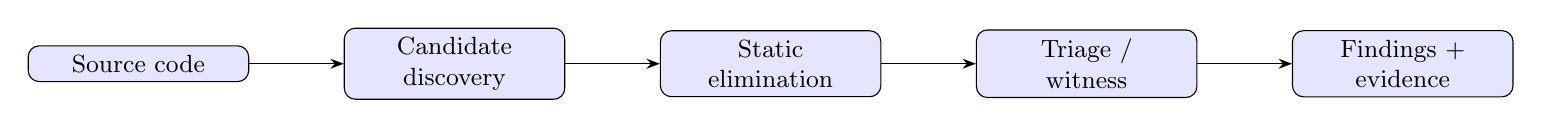
\begin{tikzpicture}[node distance=1.2cm,
  box/.style={draw, rounded corners, fill=blue!10, font=\small, minimum width=2.8cm, align=center}]
  \node[box] (src) {Source code};
  \node[box, right=of src] (disc) {Candidate\\discovery};
  \node[box, right=of disc] (elim) {Static\\elimination};
  \node[box, right=of elim] (triage) {Triage /\\witness};
  \node[box, right=of triage] (out) {Findings +\\evidence};
  \draw[-{Stealth}] (src) -- (disc);
  \draw[-{Stealth}] (disc) -- (elim);
  \draw[-{Stealth}] (elim) -- (triage);
  \draw[-{Stealth}] (triage) -- (out);
\end{tikzpicture}}%
\end{center}
\begin{itemize}
  \item \textbf{Discovery}: find every location where a bug \emph{could} occur (high recall, many FPs)
  \item \textbf{Static elimination}: prove as many candidates impossible as possible
  \item \textbf{Triage}: classify the survivors with richer context
  \item \textbf{Evidence}: attach proof artifacts or witness traces to each decision
\end{itemize}
\end{frame}

\begin{frame}{10. Paths and path conditions}
\begin{itemize}
  \item A \textbf{path} through a program is a sequence of instructions that could execute together
  \item Example: in \texttt{if x > 0: return x/y}, there are two paths:
    \begin{itemize}
      \item Path 1 (taken branch): execute \texttt{return x/y} with constraint \(x > 0\)
      \item Path 2 (not-taken branch): skip, no constraint
    \end{itemize}
  \item A \textbf{path condition} \(\Phi\) is the conjunction of all constraints that must hold for that path to execute
  \item \(\Phi = (x > 0)\) on path 1 --- only inputs satisfying this condition reach the division
  \item Key insight: if the path condition is \textbf{unsatisfiable} (\(\Phi = \text{false}\)), the path is impossible
\end{itemize}
\end{frame}

\begin{frame}[fragile]{11. A tiny worked example}
\begin{columns}
\begin{column}{0.45\textwidth}
\begin{lstlisting}[language=Python]
def f(x, y):
    if x > 0:
        return x / y  # DIV_ZERO?
    return 0
\end{lstlisting}
\end{column}
\begin{column}{0.52\textwidth}
\begin{itemize}
  \item Bug candidate: \texttt{x / y} when \(y = 0\)
  \item Path condition to reach that line: \(x > 0\)
  \item Unsafe condition: \(y = 0\)
  \item Combined: \(\Phi \wedge U \equiv (x > 0) \wedge (y = 0)\)
  \item Is this satisfiable? \textbf{Yes}: take \(x=1, y=0\)
  \item Conclusion: DIV\_ZERO is \textbf{reachable} --- real bug
\end{itemize}
\end{column}
\end{columns}
\end{frame}

\begin{frame}[fragile]{12. A guarded version of the example}
\begin{columns}
\begin{column}{0.45\textwidth}
\begin{lstlisting}[language=Python]
def f(x, y):
    if x > 0 and y != 0:
        return x / y
    return 0
\end{lstlisting}
\end{column}
\begin{column}{0.52\textwidth}
\begin{itemize}
  \item Path condition to reach division: \(x > 0 \wedge y \ne 0\)
  \item Unsafe condition: \(y = 0\)
  \item Combined: \((x > 0) \wedge (y \ne 0) \wedge (y = 0)\)
  \item Is this satisfiable? \textbf{No}: \((y \ne 0) \wedge (y = 0)\) is false
  \item Conclusion: DIV\_ZERO is \textbf{unreachable} --- false positive, eliminate it
  \item This is exactly what A3's static stage does at scale
\end{itemize}
\end{column}
\end{columns}
\end{frame}

\begin{frame}{13. The unsafe predicate family}
\begin{itemize}
  \item For each bug type \(t\), there is a predicate \(U_t(\sigma)\) that is true exactly when state \(\sigma\) represents a buggy condition
  \item Examples:
  \begin{itemize}
    \item \(U_{\text{DIV}}(\sigma) \equiv (\text{denominator}(\sigma) = 0)\)
    \item \(U_{\text{OOB}}(\sigma) \equiv (\text{index}(\sigma) \ge \text{len}(\sigma))\)
    \item \(U_{\text{NULL}}(\sigma) \equiv (\text{object}(\sigma) = \texttt{None})\)
    \item \(U_{\text{SQL}}(\sigma) \equiv (\text{taint}(\text{query}) = \texttt{user\_controlled})\)
  \end{itemize}
  \item A3 maintains 67+ such predicates covering security and reliability bug classes
  \item Each eliminates independently: prove \(R \cap U_t = \varnothing\) to kill that candidate
\end{itemize}
\end{frame}

\begin{frame}{14. What ``symbolic'' means}
\begin{itemize}
  \item \textbf{Concrete execution}: run the program with specific input values (e.g.\ \(x=3, y=7\))
  \item \textbf{Symbolic execution}: run with \emph{unknown} inputs represented as symbols (e.g.\ \(x=\alpha, y=\beta\))
  \item As the symbolic program executes, expressions build up: \texttt{z = x + 2} becomes \(z = \alpha + 2\)
  \item At a branch \texttt{if x > 0}: fork into two paths, one with constraint \(\alpha > 0\), one with \(\alpha \le 0\)
  \item Result: a tree of paths, each with a path condition, covering all inputs simultaneously
  \item A satisfiability solver then checks which paths are reachable
\end{itemize}
\end{frame}

\begin{frame}{15. Over-approximation vs under-approximation (revisited)}
\begin{itemize}
  \item When the analysis is too complex to be exact, we \textbf{approximate}
  \item \textbf{Over-approximation} (conservative): pretend the program can reach \emph{more} states than it actually can
    \begin{itemize}
      \item Risk: extra phantom states may make an unreachable bug look reachable (FP)
      \item Benefit: never misses a real bug (sound)
    \end{itemize}
  \item \textbf{Under-approximation} (optimistic): pretend the program can only reach \emph{fewer} states
    \begin{itemize}
      \item Risk: misses real bugs (FN)
      \item Benefit: everything flagged is definitely real (precise)
    \end{itemize}
  \item A3 over-approximates unknown calls conservatively; concolic under-approximates to confirm witnesses
\end{itemize}
\end{frame}

\begin{frame}{16. Counterexamples and witnesses}
\begin{itemize}
  \item A \textbf{counterexample} (to safety) is a concrete execution trace demonstrating a bug
    \begin{itemize}
      \item ``Call \texttt{f(1, 0)}: reaches line 3, divides by zero''
    \end{itemize}
  \item A \textbf{witness} to safety is a proof that no such trace exists
    \begin{itemize}
      \item ``Path condition \(\wedge\) unsafe predicate is UNSAT''
    \end{itemize}
  \item These are the two kinds of evidence A3 attaches to findings in SARIF
  \item RISE audiences care about: which kind of evidence is this finding backed by?
\end{itemize}
\end{frame}

\begin{frame}{17. The state space}
\begin{itemize}
  \item A program's \textbf{state space} is the set of all possible (program counter, variable values, heap, ...) combinations
  \item State spaces are astronomically large (or infinite)
  \item Verification's fundamental technique: reason about \textbf{sets of states} abstractly instead of individual states
  \item Many methods characterise the reachable set \(R\) implicitly via an inductive property
  \item \textbf{Key challenge}: the reachable set may be a complex shape (not a simple box/interval)
\end{itemize}
\end{frame}

\begin{frame}{18. Inductive vs non-inductive arguments}
\begin{itemize}
  \item A \textbf{non-inductive safety argument}: enumerate all paths and check each one
    \begin{itemize}
      \item Only works for programs with a finite, small number of paths
      \item Fails on loops (infinite paths)
    \end{itemize}
  \item An \textbf{inductive safety argument}: find a property \(P\) such that:
    \begin{enumerate}
      \item \(P\) holds at the start (initialisation)
      \item If \(P\) holds now and the program takes one step, \(P\) still holds (consecution)
      \item \(P\) implies safety (the unsafe states are outside \(P\))
    \end{enumerate}
  \item If you can find such a \(P\), you have proved safety for \emph{all} iterations of loops, not just finite unrollings
  \item This triple is the foundation of every method in the A3 portfolio
\end{itemize}
\end{frame}

\begin{frame}{19. The word ``consecution''}
\begin{block}{Definition}
\textbf{Consecution} (also called the \emph{inductive step}) is the property:
\[
\text{if } P(s) \text{ holds and } s \to s' \text{, then } P(s') \text{ holds}
\]
\end{block}
\begin{itemize}
  \item The name comes from ``consequence'' + ``succession'' --- the property is \emph{preserved through successive steps}
  \item You will use this word a lot in the A3 talk: ``the consecution obligation''
  \item Intuition: once you are inside the safe zone, one program step cannot throw you out
  \item If consecution holds for all transitions, the program can never escape to an unsafe state
\end{itemize}
\end{frame}

\begin{frame}{20. Why consecution is hard}
\begin{itemize}
  \item For a simple assignment \texttt{x = x + 1}, consecution check: does \(P(x) \Rightarrow P(x+1)\)?
  \item For a while loop with complex body, the transition \(s \to s'\) involves many instructions
  \item For function calls, the transition may involve unknown code (library calls)
  \item For Python: exception edges, heap mutations, dynamic dispatch all make ``one step'' complex
  \item \textbf{Main technical work} in verification is defining what ``one step'' means precisely enough to check consecution
\end{itemize}
\end{frame}

\begin{frame}{21. Safety as set separation}
\begin{itemize}
  \item Rephrase: find a set \(S\) (the ``safe zone'') such that:
  \begin{enumerate}
    \item Initial states are inside \(S\): \(S_0 \subseteq S\)
    \item \(S\) is closed under transitions: \(s \in S, s\to s' \Rightarrow s' \in S\)
    \item \(S\) and the unsafe set \(U\) do not overlap: \(S \cap U = \varnothing\)
  \end{enumerate}
  \item The set \(S\) is called an \textbf{inductive invariant}
  \item Finding such a set \emph{proves} the program is safe forever
  \item Many names for this: Lyapunov function analog, barrier certificate, loop invariant, separating predicate
\end{itemize}
\end{frame}

\begin{frame}{22. The gap between testing and verification}
\begin{center}
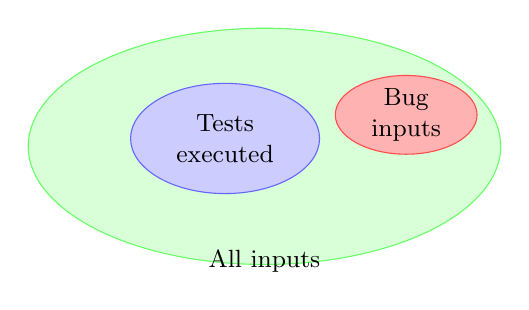
\begin{tikzpicture}
  \draw[fill=green!15, draw=green!60] (0,0) ellipse (3cm and 1.5cm) node[below=1.2cm] {\small All inputs};
  \draw[fill=blue!20, draw=blue!60] (-0.5,0.1) ellipse (1.2cm and 0.7cm) node {\small \parbox{1.8cm}{\centering Tests\\executed}};
  \draw[fill=red!30, draw=red!70] (1.8,0.4) ellipse (0.9cm and 0.5cm) node {\small \parbox{1cm}{\centering Bug\\inputs}};
\end{tikzpicture}
\end{center}
\begin{itemize}
  \item Tests cover a tiny region; bugs may live entirely outside it
  \item Verification reasoning covers the whole space (or provably excludes the red zone)
\end{itemize}
\end{frame}

\begin{frame}{23. Bug classification in A3}
\begin{itemize}
  \item A3 groups bugs into two families:
  \item \textbf{Security bugs} (taint-based): unsafe data flow from untrusted input to dangerous operation
    \begin{itemize}
      \item SQL injection, command injection, path traversal, XSS, ...
    \end{itemize}
  \item \textbf{Reliability bugs} (error-based): program state violates safety invariant at execution time
    \begin{itemize}
      \item DIV\_ZERO, INDEX\_OUT\_OF\_BOUNDS, NULL\_DEREF, UNCAUGHT\_EXCEPTION, ...
    \end{itemize}
  \item Each family uses a different unsafe predicate shape: taint predicates vs numeric/type predicates
  \item Both are handled by the same barrier/SMT machinery; only the predicate changes
\end{itemize}
\end{frame}

\begin{frame}{24. What SARIF is}
\begin{itemize}
  \item \textbf{SARIF} = Static Analysis Results Interchange Format (Microsoft/OASIS standard)
  \item A JSON format for recording analysis findings with structured evidence
  \item Key fields: rule ID, file + line, severity, confidence, message, evidence chain
  \item A3 uses SARIF to pass findings from the static stage to triage and then to CI
  \item Benefit: findings are reproducible, diffable, and queryable --- not just a text report
  \item When you say ``SARIF proof artifact'' in the talk, it means: the JSON record includes the solver outcome or certificate that justified elimination
\end{itemize}
\end{frame}

\begin{frame}{25. Chapter 1 summary: vocabulary you now know}
\begin{columns}
\begin{column}{0.48\textwidth}
\textbf{Core concepts:}
\begin{itemize}
  \item Bug, safety property, reachability
  \item True positive / false positive
  \item Path condition \(\Phi\)
  \item Unsafe predicate \(U_t\)
  \item State space, symbolic execution
\end{itemize}
\end{column}
\begin{column}{0.48\textwidth}
\textbf{Key properties:}
\begin{itemize}
  \item Soundness, completeness
  \item Over/under approximation
  \item Inductive invariant
  \item Consecution (inductive step)
  \item Counterexample, witness
\end{itemize}
\end{column}
\end{columns}
\vspace{0.3em}
\begin{block}{One-sentence summary}
Verification proves or disproves that bad states are reachable; A3 does this at scale by building
path conditions and checking them with solvers.
\end{block}
\end{frame}

%% ============================================================
%%  CHAPTER 2 — Logic, SAT, SMT, Z3
%% ============================================================

\begin{frame}{Chapter 2: Logic, SAT, and SMT Solvers}
\begin{block}{Chapter goal}
Understand what a solver is, what UNSAT means, and why Z3 is the engine behind A3's elimination step.
\end{block}
\end{frame}

\begin{frame}{26. Propositional logic in 3 minutes}
\begin{itemize}
  \item \textbf{Atoms}: Boolean variables: \(p, q, r\) (true or false)
  \item \textbf{Connectives}: \(\neg p\) (not), \(p \wedge q\) (and), \(p \vee q\) (or), \(p \Rightarrow q\) (implies)
  \item \textbf{Formula}: a combination of atoms and connectives
  \item \textbf{Assignment}: mapping each atom to true/false
  \item \textbf{Satisfying assignment}: one that makes the formula true
  \item Example: \((p \vee q) \wedge \neg p\) is satisfied by \(p=\text{false}, q=\text{true}\)
\end{itemize}
\end{frame}

\begin{frame}{27. SAT: the satisfiability problem}
\begin{block}{SAT}
Given a propositional formula \(\varphi\), is there an assignment that makes \(\varphi\) true?
\end{block}
\begin{itemize}
  \item \textbf{SAT} (Satisfiable): at least one satisfying assignment exists
  \item \textbf{UNSAT} (Unsatisfiable): no assignment makes it true --- the formula is logically impossible
  \item Example UNSAT formula: \(p \wedge \neg p\) --- requires \(p\) true and false simultaneously
  \item SAT is NP-complete, but modern SAT solvers handle millions of variables in practice
  \item SAT solvers appear everywhere in verification (IC3/PDR especially)
\end{itemize}
\end{frame}

\begin{frame}{28. From SAT to SMT}
\begin{itemize}
  \item SAT works over Boolean variables only
  \item Programs have \textbf{integers, reals, strings, arrays} --- we need richer logic
  \item \textbf{SMT} (Satisfiability Modulo Theories): SAT extended with theories for:
    \begin{itemize}
      \item \textbf{Linear arithmetic}: \(2x + 3y \le 7\), integers or reals
      \item \textbf{Nonlinear arithmetic}: \(x^2 + y^2 \le 1\)
      \item \textbf{Arrays}: \(a[i] = v\)
      \item \textbf{Bit-vectors}: \(x \mathbin{\&} 0xFF = 0\)
      \item \textbf{Strings}: regular membership, concatenation
    \end{itemize}
  \item \textbf{SMT solver}: decides satisfiability over these richer formulas
\end{itemize}
\end{frame}

\begin{frame}{29. Z3: the solver A3 uses}
\begin{itemize}
  \item \textbf{Z3} is an SMT solver developed by Microsoft Research (de Moura \& Bj\o rner, 2008)
  \item Nikolaj Bj\o rner is literally named as a target user in the project's origin story
  \item Z3 handles integer arithmetic, real arithmetic, arrays, bit-vectors, strings, and more
  \item In A3, Z3 is used to:
    \begin{enumerate}
      \item Check if \(\Phi \wedge U_t\) is satisfiable (is the bug reachable?)
      \item Solve for barrier certificate coefficients \(c_\alpha\)
      \item Check CHC constraints (consecution in interprocedural form)
    \end{enumerate}
  \item Z3 returns: \texttt{sat} + model, \texttt{unsat} + proof, or \texttt{unknown}
\end{itemize}
\end{frame}

\begin{frame}{30. What UNSAT actually means for us}
\begin{block}{When Z3 says UNSAT}
The formula \(\Phi(\sigma) \wedge U_t(\sigma)\) is \textbf{unsatisfiable}: no state can simultaneously
satisfy the path condition \emph{and} be unsafe.
\end{block}
\begin{itemize}
  \item This is a \textbf{proof of unreachability}: the bug cannot happen on this path
  \item The UNSAT proof is the ``elimination evidence'' stored in the SARIF artifact
  \item When you say ``UNSAT kills the candidate'', you mean: the solver certified impossibility
  \item UNSAT is trustworthy (up to solver correctness) --- no need for human review
\end{itemize}
\end{frame}

\begin{frame}{31. What SAT means for us}
\begin{block}{When Z3 says SAT + model}
The formula \(\Phi(\sigma) \wedge U_t(\sigma)\) is satisfiable. The model gives specific values
(e.g.\ \(x=1, y=0\)) that make both conditions true simultaneously.
\end{block}
\begin{itemize}
  \item SAT: the bug \textbf{might} be reachable (possibly after more checking)
  \item The model becomes a \textbf{witness seed} --- it specifies input values to try concretely
  \item SAT does not always mean definite bug: the symbolic model may not correspond to a real execution (spurious SAT can arise from over-approximation)
  \item Action: retain the candidate; pass model to concolic stage to confirm
\end{itemize}
\end{frame}

\begin{frame}{32. What UNKNOWN means for us}
\begin{itemize}
  \item Z3 may return \texttt{unknown} when it cannot decide within resource limits
  \item Causes: timeout, nonlinear arithmetic beyond solver's reasoning power, quantifier alternation
  \item \textbf{Conservative policy}: treat UNKNOWN as SAT --- retain the candidate, escalate to the next portfolio method
  \item This is the \textbf{soundness-preserving choice}: if we pruned on UNKNOWN, we might silently miss real bugs
  \item UNKNOWN is not a failure; it is a routing signal to a stronger/different method
\end{itemize}
\end{frame}

\begin{frame}{33. First-order logic and quantifiers}
\begin{itemize}
  \item Beyond propositional logic, we also use \textbf{first-order logic (FOL)}:
    \begin{itemize}
      \item \(\forall x: P(x)\) --- ``for all values of \(x\), property \(P\) holds''
      \item \(\exists x: P(x)\) --- ``there exists a value of \(x\) such that \(P\) holds''
    \end{itemize}
  \item The barrier certificate obligations use \(\forall\): ``for all initial states'', ``for all transitions''
  \item Z3 can handle many \(\forall\)/\(\exists\) formulas over arithmetic via quantifier instantiation
  \item Full first-order arithmetic is undecidable, which is why Z3 sometimes returns UNKNOWN
\end{itemize}
\end{frame}

\begin{frame}{34. Clauses, conjunctive normal form (CNF)}
\begin{itemize}
  \item A \textbf{clause} is a disjunction of literals: \((x > 0) \vee (y \ne 0) \vee \neg p\)
  \item \textbf{CNF} = conjunction of clauses: \(C_1 \wedge C_2 \wedge \ldots \wedge C_n\)
  \item SAT solvers work natively in CNF
  \item In IC3/PDR, the inductive invariant is maintained as a conjunction of clauses --- this is why IC3 is sometimes described as a ``clause-learning'' method
  \item When you hear ``blocking clause'' or ``proof obligation as clause'', it refers to this CNF structure
\end{itemize}
\end{frame}

\begin{frame}{35. Implications and implies-false}
\begin{itemize}
  \item \(A \Rightarrow B\) is equivalent to \(\neg A \vee B\)
  \item To prove \(A \Rightarrow \text{false}\) (i.e., \(A\) is impossible), check that \(A\) is UNSAT
  \item This is how the solver checks safety: is \((\Phi \wedge U)\) satisfiable? Equivalent to: does \(\Phi \Rightarrow \neg U\) fail?
  \item All three barrier obligations are formulated as implications checked by the solver:
    \begin{itemize}
      \item Init: \(s \in S_0 \Rightarrow B(s) \ge \epsilon\)
      \item Consec: \(B(s)\ge0 \wedge T(s,s') \Rightarrow B(s')\ge0\)
      \item Sep: \(s \in U \Rightarrow B(s) \le -\epsilon\)
    \end{itemize}
\end{itemize}
\end{frame}

\begin{frame}{36. Quantifier-free linear arithmetic (QF\_LIA / QF\_LRA)}
\begin{itemize}
  \item Most path conditions in A3 involve linear constraints (no multiplication of variables)
  \item \textbf{Quantifier-free linear integer arithmetic} (QF\_LIA): formulas like \(2x + y \le 7\)
  \item These are \textbf{decidable}: Z3 will always return SAT or UNSAT (never UNKNOWN) given enough time
  \item Most guard-based elimination in A3 falls in this decidable fragment
  \item UNKNOWN only arises from: nonlinear constraints, quantifiers over infinite domains, or timeout
\end{itemize}
\end{frame}

\begin{frame}{37. Nonlinear arithmetic and why it is hard}
\begin{itemize}
  \item \textbf{Nonlinear arithmetic}: formulas involving products of variables, e.g.\ \(x \cdot y = 0\)
  \item Polynomial arithmetic over reals (quantifier-free) is decidable (cylindrical algebraic decomposition)
    but expensive (\textsc{doubly exponential} in the number of variables)
  \item Polynomial arithmetic over integers is undecidable (related to Hilbert's 10th problem)
  \item This is why barrier certificates (which use polynomials) are expensive: they operate in nonlinear
    arithmetic land
  \item DSOS/SDSOS exist precisely to tame this cost with cheaper approximations
\end{itemize}
\end{frame}

\begin{frame}{38. What a model looks like}
\begin{itemize}
  \item When Z3 says SAT, it also returns a \textbf{model}: a concrete assignment of values
  \item Example: for \((x > 0) \wedge (y = 0) \wedge (x < 10)\), model might be \(\{x \mapsto 1, y \mapsto 0\}\)
  \item This immediately gives us \textbf{test inputs} that would trigger the bug
  \item A3's concolic stage takes this model and executes the program concretely with those values
  \item If the concrete execution actually hits the unsafe state, the bug is confirmed real
\end{itemize}
\end{frame}

\begin{frame}{39. Proof certificates from SMT solvers}
\begin{itemize}
  \item When Z3 returns UNSAT, it can optionally produce a \textbf{proof certificate}: a checkable
    derivation showing exactly which axioms and steps led to contradiction
  \item This is the mathematical guarantee that the UNSAT result is correct
  \item In practice, A3 uses the UNSAT result as evidence; full proof certificate generation is
    expensive and used selectively
  \item \textbf{UNSAT core}: a minimal subset of the input formula that is already UNSAT
    --- useful for understanding \emph{which} constraints caused the contradiction (e.g.\ which guard killed the bug)
\end{itemize}
\end{frame}

\begin{frame}{40. Craig interpolants: preview}
\begin{itemize}
  \item Given formula \(A \wedge B\) is UNSAT, a \textbf{Craig interpolant} \(I\) satisfies:
    \begin{itemize}
      \item \(A \Rightarrow I\) (the interpolant follows from A)
      \item \(I \wedge B\) is UNSAT (the interpolant contradicts B)
      \item \(I\) only uses symbols that appear in \emph{both} \(A\) and \(B\)
    \end{itemize}
  \item Intuition: \(I\) is the ``shared reason'' why \(A\) and \(B\) conflict
  \item In verification: \(A\) = path from start, \(B\) = unsafe condition; \(I\) = new safe-zone boundary predicate
  \item You will see this in slides 13f: interpolants as the tightest possible new template constraint
\end{itemize}
\end{frame}

\begin{frame}{41. Taint analysis in brief}
\begin{itemize}
  \item \textbf{Taint analysis} tracks whether data is ``tainted'' (comes from an untrusted source)
  \item \textbf{Source}: where tainted data enters (e.g.\ HTTP request parameter, file input)
  \item \textbf{Sink}: where tainted data would be dangerous (e.g.\ SQL query, shell command)
  \item \textbf{Sanitizer}: a function that cleans tainted data (e.g.\ \texttt{escape()}, \texttt{parameterize()})
  \item Taint unsafe predicate: \(U_{\text{SQL}}(\sigma) \equiv (\text{taint}(\text{arg}(\text{query})) = \text{unsanitized})\)
  \item A3 maintains a taint lattice through symbolic execution; the lattice has levels source/unsanitized/sanitized/safe
\end{itemize}
\end{frame}

\begin{frame}{42. The solver loop in A3: recap}
\begin{block}{Step-by-step solver interaction}
\begin{enumerate}
  \item Build symbolic state \(\sigma\) at candidate bug site
  \item Extract path condition \(\Phi(\sigma)\) from symbolic execution
  \item Form query: \(\Phi(\sigma) \wedge U_t(\sigma)\)
  \item Send to Z3
  \item \textbf{UNSAT}: add to eliminated set with evidence
  \item \textbf{SAT + model}: retain; seed concolic with model values
  \item \textbf{UNKNOWN}: retain; route to next portfolio stage
\end{enumerate}
\end{block}
\end{frame}

\begin{frame}{43. Why Z3 and not other solvers?}
\begin{itemize}
  \item Z3 is open-source, actively maintained, and has excellent Python bindings (\texttt{z3-solver} on PyPI)
  \item It covers the widest theory combination relevant to Python programs: integers, reals, arrays, bit-vectors, strings
  \item It supports incremental solving (add/remove constraints without restarting) --- important for efficiency in loops
  \item Alternative solvers: CVC5, MathSAT, Yices2 --- each has strengths; A3 currently uses Z3 as primary
  \item Nikolaj Bj\o rner (Z3 lead) is explicitly in the project origin story: ``Z3-builder level operational usefulness''
\end{itemize}
\end{frame}

\begin{frame}{44. Incremental solving and push/pop}
\begin{itemize}
  \item \textbf{Incremental solving}: add constraints progressively; Z3 remembers learned facts
  \item \textbf{push}: save current solver state (like a checkpoint)
  \item \textbf{pop}: restore to last checkpoint
  \item This is efficient for checking many candidates that share a common prefix
  \item Example: a function has 5 bug candidates, all under the same entry path condition.
    Push the shared \(\Phi\), check each \(U_t\) without restarting
\end{itemize}
\end{frame}

\begin{frame}{45. Theories combination: what it means in practice}
\begin{itemize}
  \item Python programs mix integers, booleans, strings, objects, and exceptions in one expression
  \item A path condition might look like: \((x > 0) \wedge (\text{isinstance}(x, \texttt{int})) \wedge (s = \texttt{"hello"} + t)\)
  \item SMT solvers handle this via \textbf{theory combination} (Nelson--Oppen method)
  \item Different theory solvers cooperate: arithmetic solver handles numeric parts; string solver handles string parts
  \item Combined solver is still sound; performance depends on how much cross-theory interaction there is
  \item A3's SymbolicValue carries a type tag (\texttt{INT}, \texttt{REAL}, \texttt{NONE}, object-id) to route constraints to the right theory
\end{itemize}
\end{frame}

\begin{frame}{46. The notion of a formula being ``valid''}
\begin{itemize}
  \item A formula \(\varphi\) is \textbf{valid} if it is true under \emph{every} assignment
  \item Equivalent to: \(\neg\varphi\) is UNSAT
  \item This is how we prove the barrier certificate obligations: to prove \(\forall s: A(s) \Rightarrow B(s)\), negate it to \(\exists s: A(s) \wedge \neg B(s)\) and ask Z3 if that is UNSAT
  \item If UNSAT: the implication is valid (the obligation holds)
  \item If SAT: the model gives a counterexample to the obligation
\end{itemize}
\end{frame}

\begin{frame}{47. SMT in one picture}
\begin{center}
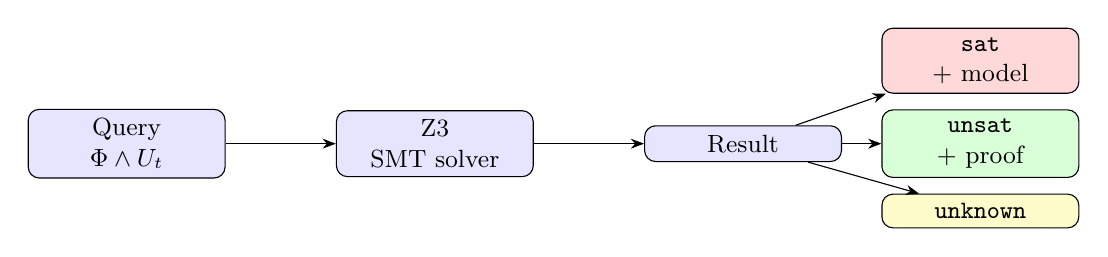
\begin{tikzpicture}[node distance=1.4cm,
  box/.style={draw, rounded corners, fill=blue!10, font=\small, align=center, minimum width=2.5cm}]
  \node[box] (q) {Query\\$\Phi \wedge U_t$};
  \node[box, right=of q] (z3) {Z3\\SMT solver};
  \node[box, right=of z3] (out) {Result};
  \node[box, above right=0.4cm and 0.5cm of out, fill=red!15] (sat) {\texttt{sat}\\+ model};
  \node[box, right=0.5cm of out, fill=green!15] (un) {\texttt{unsat}\\+ proof};
  \node[box, below right=0.4cm and 0.5cm of out, fill=yellow!20] (unk) {\texttt{unknown}};
  \draw[-{Stealth}] (q) -- (z3);
  \draw[-{Stealth}] (z3) -- (out);
  \draw[-{Stealth}] (out) -- (sat);
  \draw[-{Stealth}] (out) -- (un);
  \draw[-{Stealth}] (out) -- (unk);
\end{tikzpicture}
\end{center}
\end{frame}

\begin{frame}{48. Practical SMT pitfalls}
\begin{itemize}
  \item \textbf{Quantifier explosion}: \(\forall x\) over an infinite domain requires instantiation heuristics; can cause UNKNOWN
  \item \textbf{Nonlinear products}: \(x \cdot y\) triggers expensive procedures; prefer linear approximations where possible
  \item \textbf{Timeout}: Z3 has configurable timeouts; hitting the limit returns UNKNOWN
  \item \textbf{Encoding bugs}: if the formula does not faithfully encode the program semantics, the solver's answer is meaningless
  \item A3 invests heavily in correct encoding; every bytecode operation has a precise symbolic transfer function
\end{itemize}
\end{frame}

\begin{frame}[fragile]{49. Z3 Python API: a quick look}
\begin{lstlisting}[language=Python]
from z3 import *
x, y = Ints('x y')
solver = Solver()
solver.add(x > 0)          # path condition
solver.add(y == 0)         # unsafe predicate (DIV_ZERO)
result = solver.check()    # -> sat or unsat
if result == sat:
    print(solver.model())  # e.g. [x = 1, y = 0]
elif result == unsat:
    print("Bug unreachable - FP eliminated")
\end{lstlisting}
\begin{itemize}
  \item This is literally what A3 does for a simple guard check
  \item Real queries are much larger (hundreds of constraints from symbolic execution)
\end{itemize}
\end{frame}

\begin{frame}{50. Chapter 2 summary: solver vocabulary}
\begin{columns}
\begin{column}{0.48\textwidth}
\textbf{Logic terms:}
\begin{itemize}
  \item SAT, UNSAT, UNKNOWN
  \item SMT, Z3, theory
  \item Model (satisfying assignment)
  \item Proof certificate
  \item Valid formula
\end{itemize}
\end{column}
\begin{column}{0.48\textwidth}
\textbf{Key decisions in A3:}
\begin{itemize}
  \item UNSAT $\Rightarrow$ eliminate
  \item SAT $\Rightarrow$ retain + witness seed
  \item UNKNOWN $\Rightarrow$ retain conservatively
  \item QF\_LIA is decidable; nonlinear is hard
  \item Craig interpolant = tight new predicate from UNSAT proof
\end{itemize}
\end{column}
\end{columns}
\end{frame}

%% ============================================================
%%  CHAPTER 3 — Symbolic Execution
%% ============================================================

\begin{frame}{Chapter 3: Symbolic Execution}
\begin{block}{Chapter goal}
Learn how a verifier ``runs'' a program on abstract inputs, builds path conditions, and uses them
to check whether a bug is reachable. Understand path explosion and how A3 manages it.
\end{block}
\end{frame}

\begin{frame}[fragile]{51. Concrete vs symbolic execution: side by side}
\begin{columns}
\begin{column}{0.42\textwidth}
\textbf{Concrete run} (\(x=3\)):
\begin{lstlisting}[language=Python]
z = x + 1   # z = 4
if z > 3:   # true
  w = z * 2 # w = 8
\end{lstlisting}
\end{column}
\begin{column}{0.55\textwidth}
\textbf{Symbolic run} (\(x = \alpha\)):
\begin{lstlisting}[language=Python]
z = alpha + 1   # z = alpha+1
if z > 3:       # fork:
  # branch T: alpha+1 > 3 => alpha > 2
  w = (alpha+1)*2
  # branch F: alpha+1 <= 3 => alpha <= 2
  # skip
\end{lstlisting}
\end{column}
\end{columns}
\begin{itemize}
  \item Symbolic execution covers \textbf{all} values of \(\alpha\) in one pass
  \item Each branch gets its own path condition
\end{itemize}
\end{frame}

\begin{frame}{52. The symbolic state}
\begin{itemize}
  \item At any point in symbolic execution, the \textbf{symbolic state} records:
  \begin{itemize}
    \item \textbf{Symbolic store} \(\rho\): each variable mapped to a symbolic expression (not a value)
      e.g.\ \(\rho = \{x \mapsto \alpha, z \mapsto \alpha+1, w \mapsto 2(\alpha+1)\}\)
    \item \textbf{Path condition} \(\Phi\): conjunction of branch constraints accumulated so far
      e.g.\ \(\Phi = (\alpha > 2)\)
    \item \textbf{Program counter} \textit{pc}: which instruction executes next
  \end{itemize}
  \item At a potential bug site (e.g.\ division), extract the symbolic denominator \(d = \rho[\text{denom}]\)
  \item Bug-reachability query: is \(\Phi \wedge (d = 0)\) satisfiable?
\end{itemize}
\end{frame}

\begin{frame}{53. Branch forks and the path tree}
\begin{center}
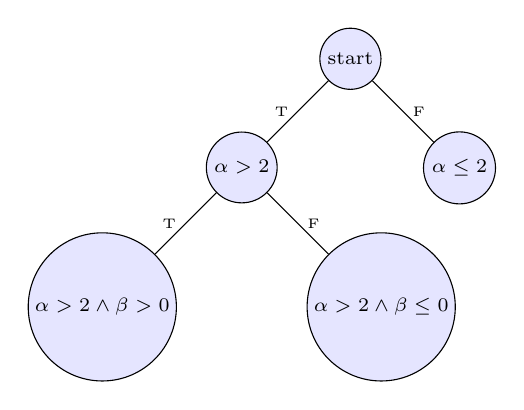
\begin{tikzpicture}[node distance=1.1cm,
  s/.style={draw, circle, fill=blue!10, inner sep=2pt, font=\scriptsize}]
  \node[s] (r) {start};
  \node[s, below left=of r] (l1) {$\alpha>2$};
  \node[s, below right=of r] (r1) {$\alpha\le2$};
  \node[s, below left=of l1] (l2) {$\alpha>2 \wedge \beta>0$};
  \node[s, below right=of l1] (r2) {$\alpha>2 \wedge \beta\le0$};
  \draw (r) -- (l1) node[midway,left,font=\tiny] {T};
  \draw (r) -- (r1) node[midway,right,font=\tiny] {F};
  \draw (l1) -- (l2) node[midway,left,font=\tiny] {T};
  \draw (l1) -- (r2) node[midway,right,font=\tiny] {F};
\end{tikzpicture}
\end{center}
\begin{itemize}
  \item Each branch doubles the number of active paths
  \item A function with \(n\) independent binary branches has up to \(2^n\) paths
  \item \textbf{Path explosion}: infeasible to enumerate all paths in a large function
\end{itemize}
\end{frame}

\begin{frame}{54. Path explosion and how to manage it}
\begin{itemize}
  \item \textbf{Loops}: potentially infinite paths (each iteration is a new fork)
  \item \textbf{Mitigations}:
    \begin{enumerate}
      \item \textbf{Loop unrolling bound}: explore at most \(k\) loop iterations (under-approximation)
      \item \textbf{Merge paths}: join states after branches with a disjunction (over-approximation)
      \item \textbf{Widening}: abstract loops into an over-approximate fixed point
      \item \textbf{Inductive invariants}: replace loop body with a proof obligation (exact but requires finding invariant)
    \end{enumerate}
  \item A3 uses loop unrolling for SMT queries and inductive barrier certificates for loops with
    infinite iteration
\end{itemize}
\end{frame}

\begin{frame}[fragile]{55. How branches become path condition constraints}
\begin{columns}
\begin{column}{0.45\textwidth}
\begin{lstlisting}[language=Python]
def f(items, idx):
    if 0 <= idx:
        if idx < len(items):
            return items[idx]
    return None
\end{lstlisting}
\end{column}
\begin{column}{0.52\textwidth}
Path to \texttt{items[idx]} (line 4):
\begin{itemize}
  \item From branch 1 (true): \(0 \le \alpha\)
  \item From branch 2 (true): \(\alpha < \text{len}(\text{items})\)
  \item Symbolic index: \(\alpha\)
  \item OOB check: \(\alpha \ge \text{len}(\text{items})\)
  \item Query: \((0 \le \alpha) \wedge (\alpha < L) \wedge (\alpha \ge L)\) = UNSAT
  \item Conclusion: access is safe, FP eliminated
\end{itemize}
\end{column}
\end{columns}
\end{frame}

\begin{frame}{56. Symbolic expressions and their representations}
\begin{itemize}
  \item A symbolic expression is a \textbf{formula tree}: leaves are symbolic variables or constants, nodes are operations
  \item Example: \texttt{(x + 2) * y - 1} becomes \((\alpha + 2) \cdot \beta - 1\) as a tree
  \item A3's \texttt{SymbolicValue} class wraps a Z3 expression
  \item Operations on \texttt{SymbolicValue} build larger Z3 expressions: \texttt{sv + 1} $\Rightarrow$ \texttt{z3\_expr + z3.IntVal(1)}
  \item The path condition \(\Phi\) is also a Z3 expression (boolean) grown with \texttt{solver.add()} calls
\end{itemize}
\end{frame}

\begin{frame}{57. Exception edges as paths}
\begin{itemize}
  \item Python is full of implicit exceptions: \texttt{TypeError}, \texttt{AttributeError}, \texttt{KeyError}, ...
  \item An exception is another kind of branch: the ``exceptional path'' vs the ``normal path''
  \item Example: \texttt{x.attr} --- two paths:
    \begin{itemize}
      \item Normal path: \(x \ne \texttt{None}\), execution continues
      \item Exception path: \(x = \texttt{None}\), \texttt{AttributeError} raised, unwinds to nearest handler
    \end{itemize}
  \item A3's symbolic execution tracks both paths; \texttt{UNCAUGHT\_EXCEPTION} is unsafe when the exception path leads out of the program with no handler
\end{itemize}
\end{frame}

\begin{frame}{58. Symbolic heap and object identity}
\begin{itemize}
  \item Python objects live on the heap; variables hold \textbf{references} (object IDs)
  \item A3 uses symbolic object IDs: variable \texttt{x} holds ID \(\iota_x\) (an integer in the symbolic store)
  \item Alias analysis: could two variables hold the same object? \(\iota_x = \iota_y\)? (can be modelled symbolically)
  \item Heap mutation (e.g.\ \texttt{x.field = v}): updates symbolic map from object-ID to field values
  \item This is expensive; A3 uses conservative approximations for complex heap structures
\end{itemize}
\end{frame}

\begin{frame}{59. Function calls in symbolic execution}
\begin{itemize}
  \item \textbf{Inlined functions}: substitute body into caller, continue symbolic execution
  \item \textbf{Summarised functions}: replace body with a pre-computed summary (pre/postcondition pair)
  \item \textbf{Unknown functions} (library calls, C extensions): use a conservative abstraction
    such as ``return any value'' or a hand-written stub
  \item A3 inlines up to a depth bound; beyond that, uses stubs or returns UNKNOWN
  \item The choice between inline/summarise affects both precision and cost
\end{itemize}
\end{frame}

\begin{frame}{60. What A3's symbolic execution engine produces}
\begin{itemize}
  \item For each function, symbolic execution produces a set of \textbf{(path condition, symbolic state)} pairs
  \item One pair per feasible path through the function body up to the bounded depth
  \item For each bug candidate \(t\) at location \(\ell\), the engine extracts:
    \begin{itemize}
      \item Which paths reach \(\ell\)?
      \item On each such path, what is the path condition?
      \item What is the symbolic value of the relevant expression (denominator, index, etc.)?
    \end{itemize}
  \item This feeds directly into the Z3 query from Chapter 2
\end{itemize}
\end{frame}

%% ============================================================
%%  CHAPTER 4 — Control Flow Graphs and Program State
%% ============================================================

\begin{frame}{Chapter 4: Control Flow Graphs and Program State}
\begin{block}{Chapter goal}
Understand CFGs, basic blocks, the state tuple, and transition systems ---
the formal foundation that A3's barrier certificate machinery is built on.
\end{block}
\end{frame}

\begin{frame}[fragile]{61. Control flow graph (CFG)}
\begin{columns}
\begin{column}{0.42\textwidth}
\begin{lstlisting}[language=Python]
def g(x):
    y = x + 1   # BB1
    if y > 0:   # BB1 end
        z = y * 2   # BB2
    else:
        z = -y      # BB3
    return z    # BB4
\end{lstlisting}
\end{column}
\begin{column}{0.55\textwidth}
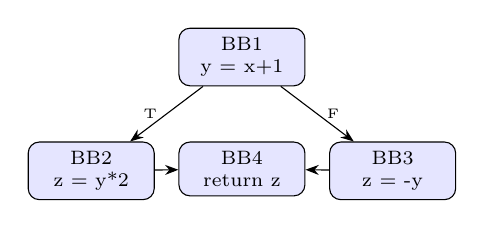
\begin{tikzpicture}[node distance=0.8cm,
  bb/.style={draw, rounded corners, fill=blue!10, font=\scriptsize, align=center, minimum width=1.6cm}]
  \node[bb] (bb1) {BB1\\y = x+1};
  \node[bb, below left=0.7cm and 0.3cm of bb1] (bb2) {BB2\\z = y*2};
  \node[bb, below right=0.7cm and 0.3cm of bb1] (bb3) {BB3\\z = -y};
  \node[bb, below=0.7cm of bb1] (bb4) {BB4\\return z};
  \draw[-{Stealth}] (bb1) -- (bb2) node[midway,left,font=\tiny]{T};
  \draw[-{Stealth}] (bb1) -- (bb3) node[midway,right,font=\tiny]{F};
  \draw[-{Stealth}] (bb2) -- (bb4);
  \draw[-{Stealth}] (bb3) -- (bb4);
\end{tikzpicture}
\end{column}
\end{columns}
\end{frame}

\begin{frame}{62. Basic blocks}
\begin{itemize}
  \item A \textbf{basic block} (BB) is a straight-line sequence of instructions with:
    \begin{itemize}
      \item Exactly one entry point (first instruction)
      \item Exactly one exit point (last instruction: conditional branch, unconditional jump, or return)
    \end{itemize}
  \item Within a basic block: no branches, no loop-backs --- execution is sequential
  \item CFG edges capture \textbf{control flow} between blocks
  \item Most analysis algorithms work at the granularity of basic blocks
\end{itemize}
\end{frame}

\begin{frame}{63. The state tuple $\sigma$}
\begin{block}{A3's program state tuple}
\[
\sigma = (\text{pc},\ \rho,\ h,\ \tau,\ \kappa,\ e,\ \Phi)
\]
\end{block}
\begin{itemize}
  \item \textbf{pc}: program counter --- which instruction is next
  \item \textbf{$\rho$}: local variable store (symbolic values)
  \item \textbf{$h$}: heap (object ID \(\to\) field values)
  \item \textbf{$\tau$}: type environment (object ID \(\to\) type)
  \item \textbf{$\kappa$}: taint tracking lattice values
  \item \textbf{$e$}: exception state (None or pending exception object)
  \item \textbf{$\Phi$}: accumulated path condition
\end{itemize}
\end{frame}

\begin{frame}{64. Transition relation}
\begin{itemize}
  \item The \textbf{transition relation} \(T(\sigma, \sigma')\) is true when the program can go from state \(\sigma\) to state \(\sigma'\) in one step
  \item Each bytecode instruction defines how \(T\) updates:
    \begin{itemize}
      \item \texttt{LOAD\_FAST x}: \(\sigma' = \sigma[\text{stack} \mathrel{+}= \rho[x]]\)
      \item \texttt{BINARY\_ADD}: \(\sigma' = \sigma[\text{stack} \mathrel{+}= v_1 + v_2]\)
      \item \texttt{POP\_JUMP\_IF\_TRUE addr}: fork two states with added constraints
    \end{itemize}
  \item The symbolic execution engine implements exactly this: apply instruction transfer functions
  \item Consecution over \(T\) is the key obligation: does the safe zone survive one step?
\end{itemize}
\end{frame}

\begin{frame}{65. Initial states $S_0$}
\begin{itemize}
  \item \(S_0\) is the set of states at the function entry point with all inputs unconstrained (fully symbolic)
  \item Formally: \(S_0 = \{(\text{pc}=\text{entry}, \rho=\text{fresh symbols}, h=\text{empty}, \ldots, \Phi=\text{true})\}\)
  \item ``\(\Phi = \text{true}$'' means: no constraints on inputs yet --- anything is possible
  \item As execution proceeds, constraints accumulate in \(\Phi\)
  \item Barrier certificates must hold for \emph{all} states in \(S_0\) --- the init obligation
\end{itemize}
\end{frame}

\begin{frame}{66. Reachable states $R$ and the fixed point}
\begin{itemize}
  \item The \textbf{reachable set} \(R\) is defined inductively:
    \[
    R_0 = S_0, \quad R_{i+1} = R_i \cup \{\sigma' : \exists \sigma \in R_i,\ T(\sigma,\sigma')\}
    \]
    \[
    R = \bigcup_{i=0}^{\infty} R_i
    \]
  \item \(R\) is the fixed point of the least-fixpoint equation: \(R = S_0 \cup \text{post}(T, R)\)
  \item For infinite-state programs (loops), \(R\) may be infinite even if the program terminates
  \item A \textbf{sound over-approximation} \(\hat{R} \supseteq R\) is sufficient to prove safety
\end{itemize}
\end{frame}

\begin{frame}{67. Why loops make reachability hard}
\begin{itemize}
  \item At a loop head, states accumulate from: entry (first pass) and back-edge (subsequent passes)
  \item After \(k\) iterations, the reachable set at the loop head is the union of \(k+1\) sets
  \item For \(k \to \infty\): the loop head reachable set requires an infinite fixed point
  \item Techniques to compute this fixed point:
    \begin{enumerate}
      \item \textbf{Widening}: aggressive over-approximation, terminates quickly but imprecise
      \item \textbf{Inductive invariant}: find a predicate \(I\) that is preserved by the loop body
      \item \textbf{Template + solver}: parameterise \(I\) by unknown coefficients; solve for them
    \end{enumerate}
  \item A3 uses template-based barrier certificates to handle loops
\end{itemize}
\end{frame}

\begin{frame}{68. Loop invariants in practice}
\begin{itemize}
  \item A \textbf{loop invariant} is a predicate \(I\) such that:
    \begin{enumerate}
      \item \(I\) holds before the loop starts (init)
      \item If \(I\) holds at the top of the loop and the body executes, \(I\) holds again at the top (consecution over the loop body)
    \end{enumerate}
  \item \(I\) also implies the property you care about at all loop exits
  \item Example: for a counting loop \texttt{for i in range(n): arr[i] = ...}, invariant \(0 \le i \le n\) ensures OOB-safety
  \item Finding \(I\) automatically is the hard problem (requires synthesis)
\end{itemize}
\end{frame}

\begin{frame}[fragile]{69. A worked loop invariant}
\begin{columns}
\begin{column}{0.4\textwidth}
\begin{lstlisting}[language=Python]
i = 0
while i < n:
    arr[i] = i * 2
    i += 1
# want: no OOB
\end{lstlisting}
\end{column}
\begin{column}{0.55\textwidth}
\textbf{Proposed invariant}: \(I \equiv (0 \le i \le n)\)
\begin{itemize}
  \item Init: \(i=0\) so \(0 \le 0 \le n\) holds (if \(n \ge 0\))
  \item Consecution: inside loop, \(i < n\) (guard), so after \(i{+}{+}\), still \(i \le n\). \(\checkmark\)
  \item Safety: \(0 \le i < n\) when accessing \texttt{arr[i]}, so no OOB. \(\checkmark\)
\end{itemize}
\emph{This is an inductive invariant that proves safety.}
\end{column}
\end{columns}
\end{frame}

\begin{frame}{70. Interprocedural analysis}
\begin{itemize}
  \item \textbf{Intraprocedural}: analyse one function in isolation (good for simple properties)
  \item \textbf{Interprocedural}: analyse across function call boundaries
  \item Why it matters: a bug often spans multiple functions:
    user input arrives in \texttt{handle\_request()}, passes through \texttt{process()}, reaches \texttt{execute\_query()} ---
    SQL injection needs full interprocedural tracking
  \item \textbf{Approach 1}: inline callees (expensive; blows up for recursive/large programs)
  \item \textbf{Approach 2}: compute \textbf{summaries} (pre/postconditions) per function; compose
  \item A3 produces per-function summaries; interprocedural taint flows use summary chaining
\end{itemize}
\end{frame}

\begin{frame}{71. Function summaries}
\begin{itemize}
  \item A \textbf{summary} for function \(f\) is a relation \(S_f(\textbf{in}, \textbf{out})\) capturing what \(f\) can do without specifying the body
  \item Example: \texttt{len(xs)} summary: \(\textbf{out} = \text{length}(\textbf{in})\), always $\ge$ 0
  \item \textbf{Modular verification}: verify each function independently using summaries of callees
  \item \textbf{Contract-based}: function contracts are a special case of summaries where developer writes them
  \item A3 can use hand-specified stubs (for library calls) and auto-inferred summaries (for project code)
\end{itemize}
\end{frame}

\begin{frame}{72. What the A3 transition system looks like precisely}
\begin{itemize}
  \item \textbf{State}: \(\sigma = (\text{pc}, \rho, h, \tau, \kappa, e, \Phi)\) as defined earlier
  \item \textbf{Initial states}: \(S_0 = \{\sigma_0\}\) where \(\sigma_0\) has fresh symbolic inputs and empty constraints
  \item \textbf{Transition}: bytecode-level small-step semantics, one instruction at a time
  \item \textbf{Unsafe predicate}: \(U_t(\sigma)\) --- depends on bug type \(t\)
  \item \textbf{Goal}: prove \(\forall \sigma \in R : \neg U_t(\sigma)\), equivalently find inductive invariant \(I\) that separates \(R\) from \(U_t\)
  \item The barrier certificate is exactly this invariant, but with a polynomial encoding that Z3 can reason about
\end{itemize}
\end{frame}

\begin{frame}{73. CFG edges: normal, exception, call, return}
\begin{center}
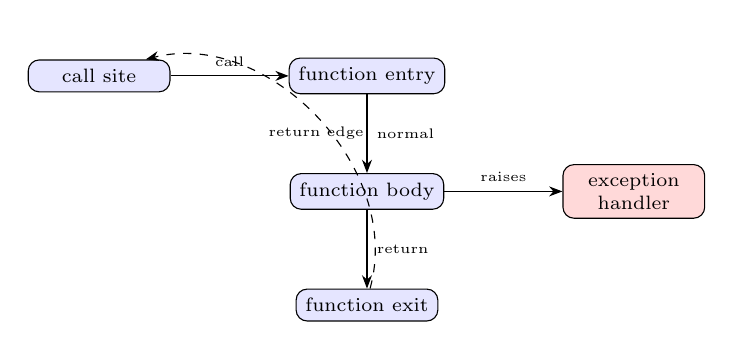
\begin{tikzpicture}[node distance=1.2cm,
  bb/.style={draw, rounded corners, fill=blue!10, font=\scriptsize, align=center, minimum width=1.8cm},
  exc/.style={draw, rounded corners, fill=red!15, font=\scriptsize, align=center, minimum width=1.8cm}]
  \node[bb] (c) {call site};
  \node[bb, right=1.5cm of c] (f) {function entry};
  \node[bb, below=1cm of f] (fb) {function body};
  \node[bb, below=1cm of fb] (fe) {function exit};
  \node[exc, right=1.5cm of fb] (ex) {exception\\handler};
  \draw[-{Stealth}] (c) -- (f) node[midway,above,font=\tiny]{call};
  \draw[-{Stealth}] (f) -- (fb) node[midway,right,font=\tiny]{normal};
  \draw[-{Stealth}] (fb) -- (fe) node[midway,right,font=\tiny]{return};
  \draw[-{Stealth}] (fb) -- (ex) node[midway,above,font=\tiny]{raises};
  \draw[-{Stealth},dashed] (fe) to[bend right=60] node[midway,below,font=\tiny]{return edge} (c);
\end{tikzpicture}
\end{center}
\begin{itemize}
  \item Exception edges are often the path through which bugs propagate
  \item A3 tracks exception paths symbolically, not just normal control flow
\end{itemize}
\end{frame}

\begin{frame}{74. Program slicing for focused analysis}
\begin{itemize}
  \item A \textbf{program slice} w.r.t.\ a bug candidate at location \(\ell\) keeps only the instructions
    that could influence the variables relevant to the bug
  \item Example: for DIV\_ZERO at \texttt{a/b}, keep only code that assigns to or affects \texttt{b}'s value
  \item \textbf{Backward slice}: walk backward through data-flow edges from \(\ell\)
  \item Slicing dramatically reduces the size of the symbolic execution problem
  \item A3 performs lightweight slicing before generating the Z3 query
\end{itemize}
\end{frame}

\begin{frame}{75. Chapter 3+4 summary: execution and state model}
\begin{columns}
\begin{column}{0.48\textwidth}
\textbf{Symbolic execution:}
\begin{itemize}
  \item Symbolic store + path condition
  \item Branch fork creates path tree
  \item Path explosion managed by bounds/invariants
  \item Exception edges are paths too
\end{itemize}
\end{column}
\begin{column}{0.48\textwidth}
\textbf{Program model:}
\begin{itemize}
  \item CFG: basic blocks + edges
  \item State tuple $(\text{pc}, \rho, h, \tau, \kappa, e, \Phi)$
  \item Transition relation $T$
  \item Reachable set $R$ = fixed point
  \item Loop $\Rightarrow$ inductive invariant needed
\end{itemize}
\end{column}
\end{columns}
\end{frame}

%% ============================================================
%%  CHAPTER 5 — Inductive Invariants and Consecution
%% ============================================================

\begin{frame}{Chapter 5: Inductive Invariants and Consecution}
\begin{block}{Chapter goal}
Master the concept of consecution deeply. Understand loop invariants, the induction pattern,
and k-induction --- the foundation of every formal proof of safety.
\end{block}
\end{frame}

\begin{frame}{76. The three-property safety proof pattern}
\begin{block}{Inductive invariant safety proof}
To prove \(S_0 \cap T^* \to U = \varnothing\), find a set \(I\) with:
\[
\underbrace{S_0 \subseteq I}_{\text{(I) Initiation}}
\quad
\underbrace{I \times I \supseteq T \cap (I \times \mathit{All})}_{\text{(C) Consecution}}
\quad
\underbrace{I \cap U = \varnothing}_{\text{(S) Separation}}
\]
\end{block}
\begin{itemize}
  \item \textbf{Initiation}: every initial state is inside \(I\)
  \item \textbf{Consecution}: the image of \(I\) under \(T\) stays inside \(I\)
  \item \textbf{Separation}: \(I\) never overlaps the unsafe region
\end{itemize}
These three properties prove that no execution can ever reach \(U\).
\end{frame}

\begin{frame}{77. Why all three obligations are necessary}
\begin{itemize}
  \item \textbf{Without Initiation}: \(I\) might be safe but the program starts outside it --- useless
  \item \textbf{Without Consecution}: \(I\) might hold at start but the program escapes \(I\) on step 2
  \item \textbf{Without Separation}: \(I\) overlaps \(U\) --- we cannot conclude the bug is unreachable
  \item Think of \(I\) as a \textbf{fence}: init says ``program starts inside the fence''; consecution says
    ``the fence is sturdy enough to keep the program in''; separation says ``the fence excludes the danger zone''
  \item All three fences must hold simultaneously
\end{itemize}
\end{frame}

\begin{frame}{78. A simple invariant example: counting}
\begin{itemize}
  \item Program: increment counter \texttt{n} from 0 to 100; check at each step that \(n \le 100\)
  \item Proposed invariant: \(I \equiv (0 \le n \le 100)\)
  \item Initiation: \(n = 0 \Rightarrow 0 \le 0 \le 100\). \checkmark
  \item Transition: \(n \to n+1\), guard is \(n < 100\)
  \item Consecution: \((0 \le n \le 100) \wedge (n < 100) \Rightarrow (0 \le n+1 \le 100)\). \checkmark
  \item Separation: \(I\) clearly avoids \(U \equiv (n > 100)\). \checkmark
  \item Proof complete --- counter never exceeds 100
\end{itemize}
\end{frame}

\begin{frame}{79. Consecution as a query}
\begin{itemize}
  \item The consecution check is: is this formula UNSAT?
  \[
  I(\sigma) \wedge T(\sigma, \sigma') \wedge \neg I(\sigma')
  \]
  \item This says: ``\(I\) holds now, the program takes one step, but \(I\) fails after the step'' ---
    if this has no solution, consecution holds
  \item Send to Z3: \texttt{solver.check(I(s) $\wedge$ T(s,s') $\wedge$ not I(s'))}
  \item If UNSAT: consecution proved
  \item If SAT: the model gives a specific pre-state and post-state that violate consecution --- a counterexample to help refine \(I\)
\end{itemize}
\end{frame}

\begin{frame}{80. The induction metaphor}
\begin{itemize}
  \item Mathematical induction: to prove \(P(n)\) for all \(n \ge 0\):
    \begin{enumerate}
      \item Prove \(P(0)\) (base case)
      \item Prove \(P(n) \Rightarrow P(n+1)\) (inductive step)
    \end{enumerate}
  \item Program inductive invariant is exactly the same:
    \begin{enumerate}
      \item Base case = Initiation: \(I\) holds at step 0
      \item Inductive step = Consecution: if \(I\) holds at step \(n\), it holds at step \(n+1\)
    \end{enumerate}
  \item The ``step'' here is one execution step of the program (one instruction or one loop iteration)
  \item This metaphor helps explain why a proof works for \emph{all} iterations of a loop, not just a bounded number
\end{itemize}
\end{frame}

\begin{frame}{81. When consecution is easy vs hard}
\begin{itemize}
  \item \textbf{Easy}: assignments with linear expressions; direct SMT query on linear arithmetic
  \item \textbf{Hard}: loops with complex nonlinear update (e.g.\ \(x \leftarrow x^2 + y\))
  \item \textbf{Hard}: heap mutations that change aliasing structure
  \item \textbf{Hard}: dynamic dispatch (which method actually runs?) --- over-approximated by considering all possible callees
  \item \textbf{Hard}: unknown side effects from unanalysed library calls
  \item A3 uses a portfolio: simple linear invariants first (fast), barrier certificates for nonlinear, UNKNOWN routing for the rest
\end{itemize}
\end{frame}

\begin{frame}{82. The simplest inductive invariant: the guard itself}
\begin{itemize}
  \item Often the simplest invariant is the \textbf{guard condition} that protects the bug
  \item Example: \texttt{if y != 0: result = x / y} --- guard is \(y \ne 0\)
  \item Proposed \(I\): ``we can only reach the division when \(y \ne 0\)'' encodes the guard in the invariant
  \item This is essentially what the path-condition check does: verify that \(\Phi \Rightarrow \neg U_t\)
  \item For more complex programs, the invariant must be synthesised because the guard is not immediately at the bug site
\end{itemize}
\end{frame}

\begin{frame}{83. k-induction: relaxing the base case}
\begin{itemize}
  \item \textbf{Simple induction} requires: \(I(\sigma) \Rightarrow I(\sigma')\)
  \item \textbf{k-induction}: prove that if \(I\) holds for \(k\) consecutive states, it holds for the \((k+1)\)-th:
    \[
    I(\sigma_0) \wedge I(\sigma_1) \wedge \ldots \wedge I(\sigma_{k-1}) \wedge T^k(\sigma_0, \sigma_k) \Rightarrow I(\sigma_k)
    \]
  \item Why? Some properties do not satisfy simple induction but do satisfy \(k\)-induction for a specific \(k\)
  \item \textbf{Example}: a property that alternates between two ``safe'' sub-states requires \(k=2\) to prove
  \item A3 can escalate from \(k=1\) to higher \(k\) when simple induction fails
\end{itemize}
\end{frame}

\begin{frame}{84. k-induction worked example}
\begin{itemize}
  \item Program: two state machine variables \(a, b\) alternating: each step \((a,b) \to (b, a+b)\)
  \item Safety property: \(a > 0 \wedge b > 0\), starting from \(a=1, b=1\)
  \item Simple induction check: \((a > 0 \wedge b > 0) \Rightarrow (b > 0 \wedge (a+b) > 0)\) --- holds! (\checkmark)
  \item So simple induction works here; some cases genuinely need \(k > 1\)
  \item Key point: \textbf{k-induction is strictly more powerful} --- it can prove properties that simple induction cannot, while being a sound technique
\end{itemize}
\end{frame}

\begin{frame}{85. Strengthening invariants}
\begin{itemize}
  \item Sometimes \(I\) fails consecution: the post-state escapes \(I\) for some transition
  \item The model (counterexample to consecution) gives a clue about what is missing
  \item \textbf{Invariant strengthening}: add an additional conjunct to \(I\) to block that counterexample
  \item Example: \(I_1 = (n \ge 0)\) fails; SAT model shows \(n = -1\) is reachable via exception path
  \item Strengthen to \(I_2 = (n \ge 0) \wedge (\text{exception} = \text{None})\)
  \item Repeat until consecution holds or we give up (UNKNOWN)
  \item This iterative strengthening is the basis of CEGAR (Chapter 7)
\end{itemize}
\end{frame}

\begin{frame}{86. The ghost of the inductive invariant: what it looks like geometrically}
\begin{center}
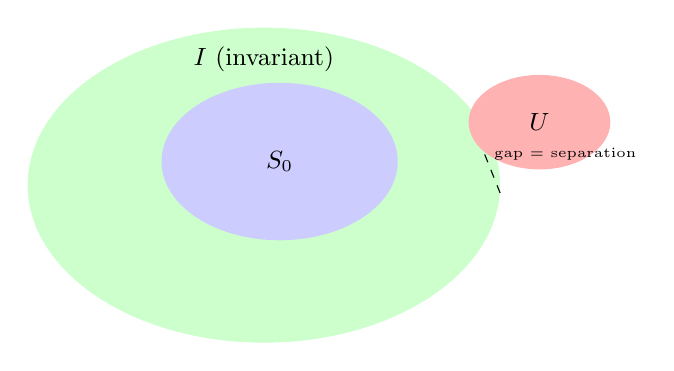
\begin{tikzpicture}
  \fill[green!20] (0,0) ellipse (3cm and 2cm);
  \fill[blue!20] (0.2,0.3) ellipse (1.5cm and 1cm);
  \fill[red!30] (3.5,0.8) ellipse (0.9cm and 0.6cm);
  \node at (0.2,0.3) {\small $S_0$};
  \node at (0,1.6) {\small $I$ (invariant)};
  \node at (3.5,0.8) {\small $U$};
  \draw[dashed] (3, -0.1) -- (2.8, 0.4) node[right,font=\tiny]{gap = separation};
\end{tikzpicture}
\end{center}
\begin{itemize}
  \item \(S_0 \subseteq I\) (initiation): small blue inside big green
  \item \(I \cap U = \varnothing\) (separation): green and red do not touch
  \item The transition keeps all reachable states inside the green ellipse
\end{itemize}
\end{frame}

\begin{frame}{87. Relationship between invariants and barrier certificates}
\begin{itemize}
  \item An \textbf{inductive invariant} is any predicate satisfying the three obligations
  \item A \textbf{barrier certificate} is a specific kind of inductive invariant where:
    \begin{itemize}
      \item The invariant is represented as \(\{s : B(s) \ge 0\}\) for a \emph{function} \(B\)
      \item \(B\) is a polynomial --- enabling sum-of-squares (SOS) methods to find and verify it
    \end{itemize}
  \item The barrier certificate is an \emph{implementation} of the inductive invariant concept
  \item You can describe it to the RISE audience as: ``we find an inductive invariant automatically using polynomial optimisation, which the solver can then certify''
\end{itemize}
\end{frame}

\begin{frame}{88. When is a simple invariant not enough?}
\begin{itemize}
  \item For linear programs (only additions, subtractions, constants) linear invariants suffice
  \item For nonlinear programs (multiplications, squares, transcendental functions) linear invariants may be too weak
  \item Example: safety of a square root function requires knowing \(x \ge 0\); a linear invariant over \(x\) works
  \item But: safety of a program with \(z = x*y\) may require invariants like \(z \le x^2 + y^2\) (nonlinear)
  \item This is where SOS polynomial templates are needed --- covered in Chapter 6
\end{itemize}
\end{frame}

\begin{frame}{89. The role of UNKNOWN in invariant finding}
\begin{itemize}
  \item If the solver cannot decide whether a proposed invariant is inductive:
    \begin{enumerate}
      \item Timeout on the consecution query
      \item Nonlinear terms beyond solver's reasoning power
    \end{enumerate}
  \item Result: UNKNOWN
  \item Policy: route to next portfolio method (e.g.\ try a richer polynomial template)
  \item If all portfolio methods return UNKNOWN: report candidate conservatively (do not call it FP)
  \item This preserves soundness: we only eliminate when we have a real proof
\end{itemize}
\end{frame}

\begin{frame}{90. Example: proving DIV\_ZERO unreachable with an invariant}
\begin{itemize}
  \item Function: compute \texttt{mean(data)} --- divides \texttt{sum} by \texttt{count}
  \item Candidate: DIV\_ZERO at \texttt{sum / count}
  \item Proposed invariant: \(I \equiv (\texttt{count} = \text{len}(\texttt{data}))\)
  \item This invariant says: count equals the number of elements processed
  \item At the division site, we also need: \(\text{len}(\texttt{data}) > 0\) (precondition of function)
  \item With both: \(\texttt{count} = \text{len}(\texttt{data}) > 0 \Rightarrow \texttt{count} > 0\) --- no DIV\_ZERO
  \item The invariant is proved inductive over the accumulation loop; separation holds given the precondition
\end{itemize}
\end{frame}

\begin{frame}{91. Contracts and preconditions}
\begin{itemize}
  \item A \textbf{precondition} is a constraint on the inputs that the caller must guarantee
  \item A \textbf{postcondition} is a constraint on the output that the callee must guarantee
  \item Together they form a \textbf{contract} (Hoare triple: \(\{P\}\ \text{program}\ \{Q\}\))
  \item In the \texttt{mean} example: precondition \(\text{len}(\texttt{data}) > 0\) is required
  \item A3 can use contracts to:
    \begin{itemize}
      \item Assume preconditions when analysing a callee (reduce over-approximation)
      \item Propagate postconditions to callers (compose summaries)
    \end{itemize}
\end{itemize}
\end{frame}

\begin{frame}{92. The Hoare triple}
\begin{block}{Hoare triple}
\(\{P\}\; C\; \{Q\}\): if precondition \(P\) holds before executing \(C\), then postcondition \(Q\) holds after
\end{block}
\begin{itemize}
  \item \textbf{Partial correctness}: assumes \(C\) terminates; only asserts \(Q\) if it does
  \item \textbf{Total correctness}: also asserts \(C\) terminates
  \item A3 targets partial correctness (it proves safety, not termination)
  \item Hoare logic is the mathematical framework behind program verification; all the barrier/invariant work is a specific way to find Hoare-style proofs automatically
\end{itemize}
\end{frame}

\begin{frame}{93. A3's consecution in pictures}
\begin{center}
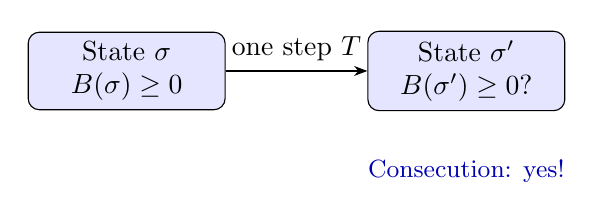
\begin{tikzpicture}[node distance=1.8cm]
  \node[draw,fill=blue!10,rounded corners,minimum width=2.5cm,align=center] (s) {State $\sigma$ \\ $B(\sigma)\ge0$};
  \node[draw,fill=blue!10,rounded corners,minimum width=2.5cm,align=center,right=of s] (sp) {State $\sigma'$ \\ $B(\sigma')\ge0$?};
  \draw[-{Stealth}] (s) -- (sp) node[midway,above]{one step $T$};
  \node[below=0.5cm of sp, font=\small, text=blue!70!black] {Consecution: yes!};
\end{tikzpicture}
\end{center}
\begin{itemize}
  \item The barrier function \(B\) assigns a non-negative score to every safe state
  \item Consecution in barrier terms: executing one step cannot make \(B\) go from $\ge0$ to $<0$
  \item Formally: \(B(\sigma) \ge 0 \wedge T(\sigma, \sigma') \Rightarrow B(\sigma') \ge 0\)
  \item This is exactly the SMT query A3 sends to Z3 for the consecution obligation
\end{itemize}
\end{frame}

\begin{frame}{94. Fixpoint operators and Kleene iteration}
\begin{itemize}
  \item Computing \(R\) exactly requires the least fixpoint of \(F(X) = S_0 \cup \text{post}(T, X)\)
  \item \textbf{Kleene iteration}: start from \(R_0 = S_0\), repeatedly apply \(F\) until no change
  \item Over finite domains: converges in finitely many steps
  \item Over infinite domains (e.g.\ integers): may never converge without widening
  \item \textbf{Widening} forces convergence by coarsening: replace an infinite ascending chain with a finite over-approximation
  \item Classic widening: widen intervals, convex hulls, etc.
\end{itemize}
\end{frame}

\begin{frame}{95. Why barrier certificates avoid the fixpoint problem}
\begin{itemize}
  \item Kleene iteration requires \emph{computing} the reachable set step by step
  \item Barrier certificate approach: directly \emph{guess} (via template) a function \(B\) that satisfies all three obligations
  \item The solver then \textbf{verifies} the three obligations by checking satisfiability --- no iteration needed
  \item This is called ``assume--verify'' or ``certificate search'': find a witness, then verify it
  \item Advantage: if the template is right, solver returns quickly
  \item Disadvantage: if no template of the given form works, the approach fails (returns UNKNOWN)
\end{itemize}
\end{frame}

\begin{frame}{96. Template-based invariant synthesis}
\begin{itemize}
  \item A \textbf{template} is a parametric form for \(B\), e.g.\ linear: \(B(\mathbf{x}) = \mathbf{c}^\top \mathbf{x} + c_0\)
  \item The unknowns are the coefficients \((c_1, \ldots, c_n, c_0)\)
  \item The three obligations become constraints on the coefficients:
    \begin{itemize}
      \item Initiation: for all \(\sigma_0 \in S_0\), \(\mathbf{c}^\top \sigma_0 + c_0 \ge \epsilon\)
      \item Consecution: for all \((\sigma, \sigma')\) with \(T(\sigma, \sigma')\), \(\mathbf{c}^\top \sigma' + c_0 \ge 0\) if \(\mathbf{c}^\top \sigma + c_0 \ge 0\)
      \item Separation: for all \(\sigma \in U\), \(\mathbf{c}^\top \sigma + c_0 \le -\epsilon\)
    \end{itemize}
  \item Solving these constraints gives the certificate coefficients
\end{itemize}
\end{frame}

\begin{frame}{97. Existential vs universal quantification in synthesis}
\begin{itemize}
  \item The synthesis problem is: \(\exists c_1, \ldots, c_n:\ \forall \sigma: \text{obligations hold}\)
  \item This is an \(\exists\forall\) problem --- harder than pure SMT (which handles \(\exists\) over fixed formula)
  \item Strategy: use \textbf{Farkas' lemma} (for linear arithmetic) or \textbf{SOS certificates} (for polynomial) to convert the \(\forall\) into a form Z3 can handle
  \item Result: the synthesis problem reduces to a single SMT query with unknown coefficients
  \item For polynomial templates, the SOS relaxation converts it to a semidefinite program (SDP) --- covered next chapter
\end{itemize}
\end{frame}

\begin{frame}{98. Summary: what eliminates a candidate}
\begin{itemize}
  \item A candidate (possible bug at location \(\ell\)) is eliminated when:
  \begin{enumerate}
    \item \textbf{Path-level UNSAT}: the path condition joining \(S_0\) to \(\ell\) with the unsafe predicate is UNSAT
    \item \textbf{Inductive invariant}: an \(I\) passing Init+Consec+Sep is found (barrier certificate is one way)
    \item \textbf{Guard discharge}: the guard protecting the bug makes \(\Phi \wedge U\) UNSAT directly
  \end{enumerate}
  \item Methods 1 and 3 are the same (path-level check); Method 2 is the barrier/invariant approach for loop-sensitive proofs
  \item A3 tries the cheaper methods first, escalates to barrier only when needed
\end{itemize}
\end{frame}

\begin{frame}{99. Chapter 5 summary: consecution vocab}
\begin{columns}
\begin{column}{0.48\textwidth}
\textbf{Core concepts:}
\begin{itemize}
  \item Inductive invariant (I)
  \item Init / Consecution / Separation
  \item Hoare triple \{P\} C \{Q\}
  \item Induction metaphor for programs
\end{itemize}
\end{column}
\begin{column}{0.48\textwidth}
\textbf{Advanced:}
\begin{itemize}
  \item k-induction
  \item Invariant strengthening
  \item Template + coefficient search
  \item Kleene iteration and widening
  \item $\exists\forall$ synthesis vs SMT
\end{itemize}
\end{column}
\end{columns}
\begin{block}{One-sentence summary}
Consecution is the inductive step: the safe zone must be closed under program transitions.
Finding it automatically requires template-based synthesis and SMT.
\end{block}
\end{frame}

\begin{frame}{100. Halfway checkpoint: what you now know}
\begin{itemize}
  \item \textbf{Ch 1}: bugs, safety, reachability, TP/FP, soundness
  \item \textbf{Ch 2}: SAT/UNSAT/UNKNOWN, Z3, SMT theories, Craig interpolants
  \item \textbf{Ch 3}: symbolic execution, path trees, path conditions, path explosion
  \item \textbf{Ch 4}: CFGs, state tuple, transition relation, loops, interprocedural
  \item \textbf{Ch 5}: inductive invariants, initiation, consecution, separation, k-induction
\end{itemize}
\vspace{0.5em}
\begin{block}{What's coming}
Ch 6: barrier certificates and SOS polynomials (the math) \quad
Ch 7: CEGAR, IC3/PDR, interpolants \quad
Ch 8: concolic execution, synthesis, confidence, CI ratchet
\end{block}
\end{frame}

%% ============================================================
%%  CHAPTER 6 — Barrier Certificates and SOS
%% ============================================================

\begin{frame}{Chapter 6: Barrier Certificates and Sum-of-Squares}
\begin{block}{Chapter goal}
Learn the central proof technique in A3: what a barrier certificate is, what the three obligations
mean in polynomial language, and why sum-of-squares (SOS) makes the problem tractable.
\end{block}
\end{frame}

\begin{frame}{101. The barrier intuition: a level-set fence}
\begin{itemize}
  \item A \textbf{barrier certificate} is a function \(B: \mathbb{R}^n \to \mathbb{R}\) such that:
  \begin{enumerate}
    \item \(B(s) \ge \epsilon > 0\) for all initial states \(s \in S_0\)
    \item \(B(s) \le -\epsilon < 0\) for all unsafe states \(s \in U\)
    \item \(B\) does not decrease across transitions: \(B(s) \ge 0 \wedge T(s,s') \Rightarrow B(s') \ge 0\)
  \end{enumerate}
  \item The level set \(\{s : B(s) = 0\}\) is a \textbf{barrier surface} separating safe from unsafe
\end{itemize}
\begin{center}
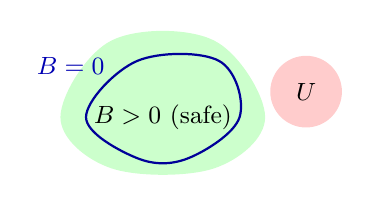
\begin{tikzpicture}[scale=0.65]
  \fill[green!20] plot[smooth cycle,tension=0.6] coordinates {(-2,0) (-1,1.5) (1,1.5) (2,0) (1,-1) (-1,-1)};
  \fill[red!20] (2.8,0.5) circle (0.7cm);
  \draw[blue!60!black, thick] plot[smooth cycle,tension=0.6] coordinates {(-1.5,0) (-0.5,1.1) (1.1,1.1) (1.5,0) (0.5,-0.8) (-0.5,-0.8)};
  \node at (0,0) {\small $B>0$ (safe)};
  \node at (2.8,0.5) {\small $U$};
  \node[text=blue!70!black] at (-1.8,1) {\small $B=0$};
\end{tikzpicture}
\end{center}
\end{frame}

\begin{frame}{102. Why a function (not just a set) is convenient}
\begin{itemize}
  \item An inductive invariant is a \emph{set}. Searching over all sets is intractable.
  \item Representing the invariant as a \textbf{function} allows parametric search:
    choose a template \(B(\mathbf{x}) = \sum_\alpha c_\alpha \mathbf{x}^\alpha\), unknown $c_\alpha$
  \item The three obligations become constraints on the coefficients \(c_\alpha\)
  \item Solve for \(c_\alpha\) $\Rightarrow$ you have the certificate
  \item \textbf{Polynomial} \(B\) is a natural choice: closed under addition and multiplication, broadly expressive, and SMT-tractable via SOS
\end{itemize}
\end{frame}

\begin{frame}{103. The three polynomial obligations}
\begin{block}{Polynomial barrier obligations}
For polynomial \(B(\mathbf{x})\) and program transitions:
\begin{align*}
\text{(Init)} &\quad \forall s \in S_0: B(s) \ge \epsilon \\
\text{(Consec)} &\quad \forall s, s': B(s)\ge0 \wedge T(s,s') \Rightarrow B(s')\ge0 \\
\text{(Sep)} &\quad \forall s \in U: B(s) \le -\epsilon
\end{align*}
\end{block}
\begin{itemize}
  \item Each obligation is a \emph{universal} statement over states
  \item Negating gives existential queries --- Z3 can check these via SMT
  \item For polynomial \(B\) and polynomial constraints, \textbf{SOS} gives a systematic way to satisfy them
\end{itemize}
\end{frame}

\begin{frame}{104. What is a polynomial?}
\begin{itemize}
  \item A \textbf{polynomial} in variables \(x_1, \ldots, x_n\) is a finite sum of \textbf{monomials}:
    \[p(\mathbf{x}) = \sum_\alpha c_\alpha \mathbf{x}^\alpha, \quad \mathbf{x}^\alpha = x_1^{\alpha_1} \cdots x_n^{\alpha_n}\]
  \item Degree of a monomial: \(\sum_i \alpha_i\)
  \item Example (\(n=2\), degree 2): \(B(x,y) = 3x^2 - 2xy + y^2 + x - 4\)
  \item A3 typically uses degree-2 polynomial templates (fast) and escalates to degree 4 if needed
  \item More monomials = more expressive invariants, but harder to solve for coefficients
\end{itemize}
\end{frame}

\begin{frame}{105. Sum-of-squares (SOS): what it means}
\begin{block}{Definition}
A polynomial \(p(\mathbf{x})\) is \textbf{sum-of-squares (SOS)} if it can be written as:
\[p(\mathbf{x}) = \sum_{i=1}^k q_i(\mathbf{x})^2\]
for polynomials \(q_i\).
\end{block}
\begin{itemize}
  \item An SOS polynomial is \emph{always} non-negative: \(p(\mathbf{x}) \ge 0\) for all \(\mathbf{x}\)
  \item NB: the converse is not always true (non-negative does not always imply SOS --- this is a famous result)
  \item But for our purposes: SOS is a sufficient certificate of non-negativity, and it can be \emph{checked efficiently}
\end{itemize}
\end{frame}

\begin{frame}{106. SOS and semidefinite programming}
\begin{itemize}
  \item \(p(\mathbf{x}) = \mathbf{m}^\top Q \, \mathbf{m}\) where \(\mathbf{m}\) is the vector of monomials and \(Q\) is a matrix
  \item \(p\) is SOS if and only if \(Q\) is \textbf{positive semidefinite} (PSD): \(Q \succeq 0\)
  \item Checking or finding a PSD \(Q\) is a \textbf{semidefinite program (SDP)} --- solvable in polynomial time
  \item This is the key: SOS reduces non-negativity (hard in general) to SDP (tractable)
  \item A3 uses an SDP solver (e.g.\ CVXPY/MOSEK) to find the certificate coefficients
\end{itemize}
\end{frame}

\begin{frame}{107. Positivstellensatz: SOS in constrained domains}
\begin{itemize}
  \item We need non-negativity not over all \(\mathbb{R}^n\) but only over the initial/unsafe sets (which are defined by polynomial inequalities)
  \item \textbf{Positivstellensatz} (Stengle, 1974): if \(p > 0\) on the set \(\{g_1 \ge 0, \ldots, g_k \ge 0\}\), then there exist SOS polynomials \(\sigma_i\) such that:
    \[p = \sigma_0 + \sigma_1 g_1 + \sigma_2 g_2 + \ldots\]
  \item This converts the constrained non-negativity into an unconstrained SOS problem
  \item \textbf{In A3}: the initial set \(S_0\) and unsafe set \(U\) are described by polynomial inequalities; Positivstellensatz makes the Init/Sep obligations solvable via SDP
\end{itemize}
\end{frame}

\begin{frame}{108. The S-procedure shortcut}
\begin{itemize}
  \item For quadratic functions on linear constraints, there is a simpler tool: the \textbf{S-procedure}
  \item Given: want to prove \(p(x) \ge 0\) whenever \(g(x) \ge 0\) (where \(p, g\) are quadratic)
  \item S-procedure: this holds if there exist \(\lambda \ge 0\) such that \(p(x) - \lambda g(x)\) is SOS
  \item This is a single SDP feasibility problem: find \(\lambda\) and the SOS decomposition
  \item Many of A3's consecution proofs for simple programs reduce to an S-procedure SDP
\end{itemize}
\end{frame}

\begin{frame}{109. Finding the barrier: the synthesis SDP}
\begin{itemize}
  \item Template: \(B(\mathbf{x}) = \mathbf{c}^\top \boldsymbol{\phi}(\mathbf{x})\) where \(\boldsymbol{\phi}\) is the vector of monomials up to degree \(d\)
  \item Obligations become linear matrix inequalities (LMIs) in the coefficients \(\mathbf{c}\):
    \begin{itemize}
      \item Init: \(\mathbf{c}^\top \boldsymbol{\phi}(\sigma_0) \ge \epsilon\) for each initial state generator
      \item Consec: via Positivstellensatz, a matrix inequality in \(\mathbf{c}\)
      \item Sep: \(\mathbf{c}^\top \boldsymbol{\phi}(u) \le -\epsilon\) for each unsafe state generator
    \end{itemize}
  \item Solve the SDP: if feasible, the solution \(\mathbf{c}^*\) gives the barrier certificate
  \item If infeasible: no barrier of the chosen degree exists; try higher degree or another method
\end{itemize}
\end{frame}

\begin{frame}{110. DSOS and SDSOS: cheaper variants}
\begin{itemize}
  \item \textbf{SOS} requires a full positive semidefinite matrix --- \(O(d^3)\) cost for degree \(d\)
  \item For large programs with many variables, this is prohibitively expensive
  \item \textbf{DSOS} (diagonally dominant SOS): restrict \(Q\) to be diagonally dominant (a sufficient condition for PSD that is a linear program, not SDP)
  \item \textbf{SDSOS} (scaled diagonally dominant SOS): slightly looser restriction, still LP-solvable
  \item DSOS/SDSOS are \textbf{sound subsets of SOS}: if DSOS finds a certificate, it is also valid under SOS
  \item Tradeoff: DSOS is faster but might miss certificates SOS would find
\end{itemize}
\end{frame}

\begin{frame}{111. Why A3 uses multiple polynomial degrees}
\begin{itemize}
  \item Degree-1 (linear): cheapest; handles programs with linear data flow; misses many real invariants
  \item Degree-2 (quadratic): handles quadratic state relationships; covers most reliable-bug patterns
  \item Degree-4 (quartic): required for programs with multiplication of program variables
  \item A3 starts with degree-2 and escalates to degree-4 only if degree-2 returns infeasible
  \item Cost: number of monomials in \(n\) variables of degree \(\le d\) is \(\binom{n+d}{d}\), which grows fast
\end{itemize}
\end{frame}

\begin{frame}{112. Connecting barrier certificates to the A3 talk}
\begin{itemize}
  \item When you say ``the kitchensink tries multiple solvers'' in the talk, barrier certificates are \textbf{one of those solvers}
  \item Specifically: A3 has a ``BarrierSolver'' module that implements the SDP-based synthesis
  \item When a path-level UNSAT check fails (UNKNOWN or SAT), A3 tries to find a barrier certificate
  \item If barrier synthesis succeeds: FP eliminated with an inductive proof
  \item If barrier synthesis fails/unknown: escalate further (DSE, Houdini, etc.)
  \item The barrier solver is the ``formal certification'' layer --- the most rigorous elimination method
\end{itemize}
\end{frame}

\begin{frame}{113. Barrier certificate example: DIV\_ZERO}
\begin{itemize}
  \item Program computes \texttt{result = total / count} at end of accumulation loop
  \item State space: \((total, count)\) where count is incremented each iteration
  \item Initial state: \((0, 0)\); loop increments count each iteration
  \item Unsafe: \(count = 0\) at the division site
  \item \textbf{Barrier}: \(B(total, count) = count - \tfrac{1}{2}\)
    \begin{itemize}
      \item Init: initially \(count = 0\) --- but the loop must have been entered before division is reached. Context: division only reachable after at least 1 iteration $\Rightarrow$ \(count \ge 1\) at that point
      \item Sep: \(count = 0 \Rightarrow B = -\tfrac{1}{2} < 0\). \checkmark
      \item Consec: \(count \ge \tfrac{1}{2}\) plus the loop increment $\Rightarrow B$ stays $\ge 0$. \checkmark
    \end{itemize}
\end{itemize}
\end{frame}

\begin{frame}{114. Limitations of barrier certificates}
\begin{itemize}
  \item \textbf{Discrete programs}: SOS is designed for continuous domains; discrete (integer) jumps require adaptation
  \item \textbf{Complex control flow}: exception edges, dynamic dispatch make the transition relation hard to encode as polynomial
  \item \textbf{Template choice}: if the right degree is not tried, the method returns infeasible incorrectly
  \item \textbf{Scalability}: for programs with 50+ symbolic variables, SDP becomes slow
  \item A3 addresses these by: encoding integers as bounded reals; abstracting complex control; trying multiple degrees; using DSOS for large programs
\end{itemize}
\end{frame}

\begin{frame}{115. Prajna and Jadbabaie (2004): origin of barrier certificates}
\begin{itemize}
  \item Prajna \& Jadbabaie introduced barrier certificates for continuous dynamical systems in 2004 (HSCC)
  \item Original setting: differential equations \(\dot{x} = f(x)\); barrier function must satisfy \(\dot{B} \ge 0\) wherever \(B = 0\)
  \item A3 adapts this to discrete programs: replace \(\dot{B} \ge 0\) with $B(s')\ge0$ given $B(s)\ge0$
  \item The discrete version is more natural for programs; the key insight (level-set fence) transfers directly
  \item You can cite this as context: ``barrier certificates were originally invented for control systems; we apply the same principle to Python programs''
\end{itemize}
\end{frame}

\begin{frame}{116. Chapter 6 summary: barrier certificate vocab}
\begin{columns}
\begin{column}{0.48\textwidth}
\textbf{Core concepts:}
\begin{itemize}
  \item Barrier function $B$
  \item Level set / barrier surface
  \item Init / Consec / Sep obligations
  \item Polynomial template + degree
  \item Monomials and coefficients
\end{itemize}
\end{column}
\begin{column}{0.48\textwidth}
\textbf{Algebraic machinery:}
\begin{itemize}
  \item SOS = sum of squares
  \item SDP = semidefinite program
  \item Positivstellensatz
  \item DSOS / SDSOS variants
  \item S-procedure for quadratics
\end{itemize}
\end{column}
\end{columns}
\end{frame}

%% ============================================================
%%  CHAPTER 7 — CEGAR, IC3/PDR, Interpolants
%% ============================================================

\begin{frame}{Chapter 7: CEGAR, Abstraction, IC3/PDR, and Interpolants}
\begin{block}{Chapter goal}
Learn counterexample-guided abstraction refinement (CEGAR), the IC3/PDR incremental invariant
builder, and Craig interpolants. These are the ``repair loop'' methods when simple proofs fail.
\end{block}
\end{frame}

\begin{frame}{117. The abstraction-refinement idea}
\begin{itemize}
  \item \textbf{Problem}: full symbolic execution is too expensive; simplified models (abstractions) are cheap but imprecise
  \item \textbf{Observation}: if analysis on the \emph{abstract} model says ``no bug'', the real program is also safe (if abstraction is sound over-approximation)
  \item \textbf{Problem}: the abstract model might say ``bug possible'' when it is only a phantom of the abstraction, not real
  \item \textbf{Solution}: use the spurious counterexample to \emph{refine} the abstraction, then retry
  \item This cycle --- abstract, analyse, refine --- is \textbf{CEGAR}
\end{itemize}
\end{frame}

\begin{frame}{118. CEGAR: counterexample-guided abstraction refinement}
\begin{center}
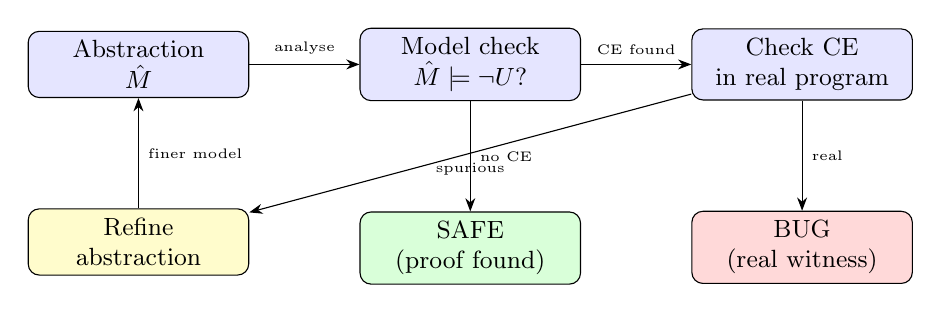
\begin{tikzpicture}[node distance=1.4cm,
  box/.style={draw,rounded corners,fill=blue!10,font=\small,align=center,minimum width=2.8cm}]
  \node[box] (abs) {Abstraction \\ $\hat{M}$};
  \node[box, right=of abs] (mc) {Model check \\ $\hat{M} \models \neg U$?};
  \node[box, below=of mc, fill=green!15] (done) {SAFE \\ (proof found)};
  \node[box, right=of mc] (ce) {Check CE \\ in real program};
  \node[box, below=of ce, fill=red!15] (bug) {BUG \\ (real witness)};
  \node[box, below=of abs, fill=yellow!20] (ref) {Refine \\ abstraction};
  \draw[-{Stealth}] (abs) -- (mc) node[midway,above,font=\tiny]{analyse};
  \draw[-{Stealth}] (mc) -- (done) node[midway,right,font=\tiny]{no CE};
  \draw[-{Stealth}] (mc) -- (ce) node[midway,above,font=\tiny]{CE found};
  \draw[-{Stealth}] (ce) -- (bug) node[midway,right,font=\tiny]{real};
  \draw[-{Stealth}] (ce) -- (ref) node[midway,below,font=\tiny]{spurious};
  \draw[-{Stealth}] (ref) -- (abs) node[midway,right,font=\tiny]{finer model};
\end{tikzpicture}
\end{center}
\end{frame}

\begin{frame}{119. What makes a counterexample spurious?}
\begin{itemize}
  \item The abstract model \(\hat{M}\) over-approximates the real program \(M\)
  \item A path in \(\hat{M}\) leading to \(U\) may not correspond to any path in \(M\)
  \item \textbf{Spurious counterexample}: the abstract CE path has no real execution trace
  \item Detection: run the CE path symbolically on the real program; if the path condition becomes UNSAT before reaching \(U\), it is spurious
  \item Spurious CE gives valuable information: the abstract path was infeasible \emph{for a reason} --- extract that reason as a new abstraction predicate
\end{itemize}
\end{frame}

\begin{frame}{120. Predicate abstraction}
\begin{itemize}
  \item \textbf{Predicate abstraction}: abstract the program state by a finite set of predicates \(\{p_1, \ldots, p_k\}\)
  \item Abstract state: a boolean vector recording which predicates are true
  \item Example: predicates \(\{x > 0, y \ne 0, z < 10\}\) --- abstract state has \(2^3 = 8\) elements
  \item Transition in the abstract model: which combinations of predicate truth values are reachable in one step?
  \item Starting with coarse predicates (e.g.\ just \{true\}): fast but imprecise
  \item After CEGAR refinement: predicates grow more specific; abstraction becomes tighter
\end{itemize}
\end{frame}

\begin{frame}{121. How a spurious CE leads to a new predicate}
\begin{itemize}
  \item Spurious CE path: states \(\sigma_0 \to \sigma_1 \to \ldots \to \sigma_k\) in abstract model, but infeasible in real model
  \item The infeasibility is witnessed by an UNSAT proof: \(\Phi_0 \wedge T_1 \wedge \ldots \wedge T_k \wedge U\) is UNSAT
  \item \textbf{Interpolant extraction}: compute Craig interpolant sequence \(I_1, \ldots, I_{k-1}\) from the UNSAT proof
  \item Each \(I_i\) is a predicate over the relevant variables at step \(i\) --- it is a new ``distinguishing fact''
  \item Add these predicates to the abstraction: the refined model \emph{cannot} reproduce the spurious path
  \item Repeat until no spurious CEs remain or a real CE is found
\end{itemize}
\end{frame}

\begin{frame}{122. Craig interpolants: the formal definition}
\begin{block}{Craig interpolant}
Given \(A \wedge B\) is UNSAT, the Craig interpolant \(I\) satisfies:
\begin{enumerate}
  \item \(A \models I\) \quad (A implies I)
  \item \(I \wedge B\) is UNSAT \quad (I is incompatible with B)
  \item \(I\) uses only symbols common to \(A\) and \(B\)
\end{enumerate}
\end{block}
\begin{itemize}
  \item Intuition: \(I\) is the ``minimal shared reason'' why \(A\) rules out \(B\)
  \item In CEGAR: \(A\) = prefix of spurious path, \(B\) = suffix reaching unsafe; \(I\) = fact true after prefix that blocks the suffix
  \item Interpolant algorithms extract \(I\) from the UNSAT proof structure (proof of resolution)
\end{itemize}
\end{frame}

\begin{frame}{123. CEGAR in the A3 context}
\begin{itemize}
  \item A3 does not run a full CEGAR loop as a standalone pass (that is ModelChecking-style)
  \item Instead, CEGAR principles appear in:
    \begin{enumerate}
      \item \textbf{Template refinement}: if barrier certificate fails, use the failed-obligation model to extract new monomials to add to the template
      \item \textbf{DSE path feedback}: concolic execution finds new constraints; fed back to re-query solver with richer path condition
      \item \textbf{Houdini weakening}: start with strongest invariant candidate, weaken on counterexample
    \end{enumerate}
  \item When you mention CEGAR in the talk, this is the context: iterative refinement of what-we-know based on solver feedback
\end{itemize}
\end{frame}

\begin{frame}{124. IC3/PDR: the modern verifier's algorithm}
\begin{itemize}
  \item \textbf{IC3} (Incremental Construction of Inductive Clausal Invariants; Bradley 2011) also called \textbf{PDR} (Property Directed Reachability)
  \item Instead of searching for a global invariant, IC3 incrementally builds a \emph{frame sequence} \(F_0, F_1, \ldots, F_k\) such that:
    \begin{itemize}
      \item \(F_0 = S_0\) (initial states)
      \item Each \(F_i \supseteq F_{i+1}\) (monotone tightening)
      \item \(F_k \cap U = \varnothing\) (safety of the last frame)
      \item Each \(F_i\) is inductive relative to \(F_{i-1}\)
    \end{itemize}
  \item When two consecutive frames converge (\(F_k = F_{k+1}\)), we have found an inductive invariant
\end{itemize}
\end{frame}

\begin{frame}{125. IC3 frames as clause sets}
\begin{itemize}
  \item Each frame \(F_i\) is represented as a \textbf{conjunction of clauses} (like an CNF formula)
  \item A \textbf{clause} \(c\) in frame \(F_i\) asserts: ``no state in \(F_i\) satisfies the negation of \(c\)''
  \item When IC3 finds a state \(s\) in \(F_i\) that \emph{could} lead to \(U\), it \textbf{blocks} \(s\) by adding a new clause to \(F_{i-1}\)
  \item The blocking clause is derived by generalising \(s\) into a cube (a conjunction of literals), then negating it
  \item This process propagates blocking obligations backward through frames: ``what predecessors could lead here?''
\end{itemize}
\end{frame}

\begin{frame}{126. IC3 algorithm sketch}
\begin{enumerate}
  \item Check if \(S_0 \cap U \ne \varnothing\): if so, immediate bug at step 0
  \item Check if a predecessor of \(U\) can be in \(S_0\) (1-step reachability check)
  \item If yes: counterexample found (or generalise and block)
  \item If no: create new frame \(F_{k+1} = \{U^c\}\) (starts as ``not unsafe''); propagate clauses
  \item For each clause in \(F_i\): try to push (propagate) it to \(F_{i+1}\) by checking inductiveness
  \item If a clause propagates to \(F_{k+1}\): extend the frame sequence
  \item If convergence: invariant found; if bug trace: real CE
\end{enumerate}
\begin{itemize}
  \item Key: each SAT call either finds a CE to block or proves a clause advances
\end{itemize}
\end{frame}

\begin{frame}{127. PDR for software: CHC formulation}
\begin{itemize}
  \item IC3/PDR was originally for hardware (finite bit-vectors)
  \item For software: use \textbf{Constrained Horn Clauses (CHC)} as the formulation
  \item A CHC is a clause of the form: \(B_1(\mathbf{x}_1) \wedge \ldots \wedge B_k(\mathbf{x}_k) \wedge \phi \Rightarrow H(\mathbf{y})\)
  \item \textbf{Horn clauses} model recursive functions and loops naturally: the predicate symbol \(H\) plays the role of the loop invariant
  \item Solving a CHC system = finding interpretations for all uninterpreted predicates such that all clauses hold
  \item This is exactly the ``find the inductive invariant'' problem in Horn clause form
\end{itemize}
\end{frame}

\begin{frame}{128. SeaHorn: CHC solving for programs}
\begin{itemize}
  \item \textbf{SeaHorn} is a verification framework that encodes C/C++ programs as CHC systems and solves them
  \item A3 adopts a similar CHC encoding for Python interprocedural analyses
  \item Each function's pre/postcondition becomes a Horn clause; recursive calls become head predicates
  \item A CHC solver (e.g.\ Spacer inside Z3) then finds the invariant interpretations
  \item Benefit: CHC solving separates the ``program encoding'' from the ``invariant finding'' --- each can improve independently
  \item Spacer inside Z3 is a PDR-style CHC solver; A3 can invoke it directly
\end{itemize}
\end{frame}

\begin{frame}{129. The SLAM project and predicate abstraction at scale}
\begin{itemize}
  \item \textbf{SLAM} (Microsoft, Ball \& Rajamani, 2002) was the first large-scale CEGAR-based verifier
  \item Verified device driver property violations in Windows kernel
  \item Key technique: predicate abstraction + CEGAR, fully automated
  \item SLAM's insight: the right predicates come from the code itself (variable guards, comparisons at branches)
  \item A3's approach to predicate discovery follows the same heuristic: use branch conditions and comparison predicates from the function's own source
\end{itemize}
\end{frame}

\begin{frame}{130. Lazy abstraction and impact}
\begin{itemize}
  \item \textbf{Lazy abstraction} (Henzinger et al., 2002): do not build the full abstract program upfront;
    refine \emph{only the parts of the abstract model that were actually traversed by the CE path}
  \item Benefit: avoids refining parts of the program that are irrelevant to the current bug
  \item Result: dramatically fewer CEGAR iterations needed in practice
  \item BLAST (Berkeley Lazy Abstraction Software verification Tool) demonstrated this on real C programs
  \item A3 applies a similar ``on-demand refinement'' philosophy: only deepen analysis along paths that need it
\end{itemize}
\end{frame}

\begin{frame}{131. Chapter 7a summary: CEGAR and interpolants}
\begin{columns}
\begin{column}{0.48\textwidth}
\textbf{Core concepts:}
\begin{itemize}
  \item Abstraction / spurious CE
  \item CEGAR loop
  \item Predicate abstraction
  \item Interpolant = shared reason for UNSAT
\end{itemize}
\end{column}
\begin{column}{0.48\textwidth}
\textbf{Major systems:}
\begin{itemize}
  \item SLAM (Windows drivers)
  \item BLAST (lazy abstraction)
  \item IC3/PDR (frame-based)
  \item CHC + SeaHorn + Spacer
\end{itemize}
\end{column}
\end{columns}
\end{frame}

\begin{frame}{132. IC3 in the A3 portfolio: what role it plays}
\begin{itemize}
  \item A3's kitchensink portfolio includes an IC3/PDR-style invariant builder for cases where:
    \begin{itemize}
      \item The barrier SDP is infeasible (no polynomial certificate exists at that degree)
      \item The path condition is satisfiable but all simple guards fail
    \end{itemize}
  \item IC3 builds clause-based invariants using the Z3 SAT/UNSAT feedback loop
  \item IC3 does not need a polynomial template --- it infers the invariant structure from blocking cubes
  \item Limitation: works best on linear arithmetic; harder for nonlinear programs
  \item In practice: IC3 often handles the cases the SOS certificate misses, and vice versa
\end{itemize}
\end{frame}

\begin{frame}{133. Interpolant-based template expansion}
\begin{itemize}
  \item When the barrier SDP is infeasible with monomials \(\{1, x, y, x^2, xy, y^2\}\):
    maybe the right invariant needs term \(x^2 y\) or some other monomial not in the template
  \item Strategy: run a CEGAR step; get the failed-consecution model \((\sigma, \sigma')\)
  \item Compute interpolant between \(\Phi_0(\sigma) \wedge T(\sigma,\sigma')\) and \(\neg B(\sigma')\)
  \item Interpolant uses a new predicate structure suggesting which new monomials to add to the template
  \item Add those monomials; re-run SDP --- often finds the certificate on the second try
  \item This is the ``CEGAR inside barrier synthesis'' loop mentioned in slides 13f
\end{itemize}
\end{frame}

\begin{frame}{134. k-induction and IC3: the relationship}
\begin{itemize}
  \item \(k\)-induction checks: given the last \(k\) states all satisfy \(P\), does the next state satisfy \(P\)?
  \item IC3 generalises \(k\)-induction: frames \(F_0, \ldots, F_k\) capture exactly what holds after at most \(k\) steps
  \item IC3 dynamically determines the right \(k\) --- it is an \textbf{adaptive} induction depth finder
  \item When k-induction returns UNKNOWN at depth \(k\), IC3 can continue to depth \(k+1\) by extending the frame sequence
  \item This makes IC3 more powerful than fixed \(k\)-induction configurations
\end{itemize}
\end{frame}

\begin{frame}{135. Abstract interpretation: a brief overview}
\begin{itemize}
  \item \textbf{Abstract interpretation} (Cousot \& Cousot, 1977) is the theoretical framework behind most static analysers
  \item Key idea: define a \textbf{Galois connection} between concrete and abstract domains
  \item Abstract domain examples:
    \begin{itemize}
      \item \textbf{Interval domain}: variable \(x\) tracked as range \([l, u]\)
      \item \textbf{Octagon domain}: pairs of variables: \(\pm x \pm y \le c\)
      \item \textbf{Polyhedra domain}: conjunctions of linear inequalities
    \end{itemize}
  \item Analysing a program in the abstract domain by propagating abstract values is fast but imprecise
  \item A3 uses interval-like approximations for variable ranges before escalating to SMT/barrier
\end{itemize}
\end{frame}

\begin{frame}{136. Widening in abstract interpretation}
\begin{itemize}
  \item At a loop back-edge, abstract values grow with each iteration (e.g.\ interval \([0,1], [0,2], [0,3], \ldots \to [0, \infty)\))
  \item \textbf{Widening} operator\(\nabla\): forces convergence by extrapolating to the limit
  \item Example: \([0,1] \nabla [0,3] = [0, +\infty]\) --- widen the upper bound to infinity
  \item After widening: run \textbf{narrowing} to tighten the result: \([0, +\infty] \triangle [0,100] = [0, 100]\)
  \item Widening preserves soundness (over-approximation) but loses precision
  \item A3 uses abstract interpretation results as an initial over-approximation; SMT/barrier refine where needed
\end{itemize}
\end{frame}

\begin{frame}{137. Connecting to the RISE talk: the kitchensink portfolio}
\begin{itemize}
  \item The A3 ``kitchensink'' is the ordered portfolio of methods tried for each candidate:
  \begin{enumerate}
    \item \textbf{Guard check}: direct UNSAT on \(\Phi \wedge U_t\) (cheapest)
    \item \textbf{Abstract interpretation}: interval / octagon over-approximation (fast)
    \item \textbf{Barrier certificate} (SOS/DSOS): degree-2 --- inductive polynomial invariant
    \item \textbf{IC3/PDR clause learning}: clause-based invariant builder
    \item \textbf{k-induction}: \(k\in\{1,2,4\}\) unrolling
    \item \textbf{CEGAR loop}: predicate abstraction + interpolant refinement
    \item \textbf{DSE}: concolic confirmation (see Chapter 8)
  \end{enumerate}
  \item Each step escalates cost; the system stops at first SAFE or UNSAFE conclusion
\end{itemize}
\end{frame}

\begin{frame}{138. When every portfolio method returns UNKNOWN}
\begin{itemize}
  \item All portfolio methods exhausted; none proved safe or found a real bug
  \item Policy: retain candidate with confidence score = ``LOW'' (high uncertainty)
  \item Report in SARIF with evidence chain showing which methods were tried
  \item \textbf{Agentic triage}: a language model examines the SARIF, the code context, and assigns a final
    severity label based on contextual reasoning
  \item The triage agent looks for: Is this reachable in production context? Are there upstream guards?
    Is the code path exercised in tests?
  \item UNKNOWN survivors after triage become the ``genuine uncertainty'' report --- not suppressed
\end{itemize}
\end{frame}

\begin{frame}{139. Summary: the methods and what they prove}
\begin{center}
\begin{tabular}{lll}
\textbf{Method} & \textbf{Proves} & \textbf{Cost} \\ \hline
Path UNSAT & No bug on one path & Cheapest \\
AI / Interval & Unreachable by range & Fast \\
Barrier (SOS) & Inductive poly invariant & Medium \\
IC3/PDR & Clause invariant & Medium \\
k-Induction & Property up to depth $k$ & Scales with $k$ \\
CEGAR & Predicate abstraction & Iterative \\
Concolic (DSE) & Confirms real witness & Medium \\
\end{tabular}
\end{center}
\end{frame}

\begin{frame}{140. Chapter 7 summary: the refinement methods}
\begin{columns}
\begin{column}{0.48\textwidth}
\textbf{CEGAR:}
\begin{itemize}
  \item Abstract $\to$ analyse $\to$ check CE $\to$ refine
  \item Predicate abstraction
  \item Interpolants from UNSAT proof
  \item Lazy: refine only what matters
\end{itemize}
\end{column}
\begin{column}{0.48\textwidth}
\textbf{IC3/PDR:}
\begin{itemize}
  \item Frame sequence $F_0, \ldots, F_k$
  \item Blocking cubes from SAT models
  \item Convergence = invariant
  \item CHC generalisation for software
\end{itemize}
\end{column}
\end{columns}
\end{frame}

%% ============================================================
%%  CHAPTER 8 — Concolic Execution
%% ============================================================

\begin{frame}{Chapter 8: Concolic Execution and DSE}
\begin{block}{Chapter goal}
Learn what ``concolic'' means, how it combines concrete and symbolic execution to confirm or
refute bug witnesses, and how A3 uses it as the final gate before reporting a true positive.
\end{block}
\end{frame}

\begin{frame}{141. What ``concolic'' means}
\begin{itemize}
  \item \textbf{Concolic} = \textbf{con}crete + \textbf{sym}bolic execution, running simultaneously
  \item Coined for the DART tool (Godefroid, Klarlund, Sen, 2005)
  \item \textbf{Concrete pass}: run the program with actual input values --- fast, no approximation
  \item \textbf{Symbolic pass}: simultaneously track symbolic expressions alongside concrete values
  \item At branches: the concrete value determines which branch to take; the symbolic side records the constraint
  \item Result: one complete concrete trace paired with its exact path condition
\end{itemize}
\end{frame}

\begin{frame}{142. Why concolic avoids path explosion}
\begin{itemize}
  \item Pure symbolic execution forks at every branch: exponential paths
  \item Concolic only follows \textbf{one path} at a time (the concrete execution determines the path)
  \item After one run, \textbf{negate one branch condition} to get a new input that takes a different path
  \item Repeat: explore the unexplored branches systematically (like a guided DFS over the path tree)
  \item This is \textbf{dynamic symbolic execution (DSE)}: symbolic + driven by concrete runs
  \item Key advantage: no spurious paths --- every explored path is a real execution
\end{itemize}
\end{frame}

\begin{frame}[fragile]{143. Concolic execution step by step}
\begin{enumerate}
  \item Start with some concrete input (e.g.\ \(x=0, y=1\)) and symbolic variables \((\alpha, \beta)\)
  \item Execute concretely: \(x=0\) takes the false branch of \texttt{if x > 0}
  \item Record path condition: \(\Phi = (\alpha \le 0)\)
  \item \textbf{Negate last constraint}: \(\alpha > 0\) --- ask solver for model: \(x = 1\)
  \item Re-run with \(x=1\): now takes the true branch; new path condition \(\Phi = (\alpha > 0)\)
  \item Continue negating branches to explore the full path tree systematically
\end{enumerate}
\begin{itemize}
  \item Each iteration discovers a new path; solver generates the input that triggers it
\end{itemize}
\end{frame}

\begin{frame}{144. Concolic as witness confirmation in A3}
\begin{itemize}
  \item When SMT returns SAT with model \((x=v_1, y=v_2, \ldots)\), A3 knows: \emph{symbolically}, the bug is reachable
  \item But: due to over-approximation, the symbolic model might not correspond to a real execution
  \item A3 seeds the concolic engine with the SAT model as the starting concrete input
  \item Concolic runs the program concretely with those values
  \item If the bug is hit: \textbf{real TP} --- report with the concrete trace as evidence
  \item If the bug is not hit (path diverges): the SAT model was spurious; discard, try next portfolio step
\end{itemize}
\end{frame}

\begin{frame}{145. The concolic trace as evidence}
\begin{itemize}
  \item A confirmed concolic trace is maximally actionable evidence for a developer:
    \begin{itemize}
      \item Exact input values that trigger the bug
      \item Stack trace showing which function calls led to the bug site
      \item Variable values at each frame
    \end{itemize}
  \item A3 encodes this evidence in the SARIF record under the \texttt{codeFlows} field
  \item A developer can reproduce the bug by simply running the program with the provided inputs
  \item This sharply reduces the ``I can't reproduce it'' back-and-forth between security team and developer
\end{itemize}
\end{frame}

\begin{frame}{146. Path divergence and why it happens}
\begin{itemize}
  \item \textbf{Path divergence}: the concrete execution takes a different branch than the symbolic model predicted
  \item Causes:
    \begin{itemize}
      \item \textbf{Imprecise modelling}: symbolic model over-approximated a library call differently than reality
      \item \textbf{Environment effects}: file system, time, random number generator --- not modelled symbolically
      \item \textbf{Type mismatches}: Python dynamic typing means an object can be a different type at runtime vs the assumption made symbolically
    \end{itemize}
  \item When divergence occurs: the concrete and symbolic states differ; A3 detects this and flags the candidate as ``inconclusive'' (UNKNOWN)
\end{itemize}
\end{frame}

\begin{frame}{147. DSE coverage: exploring new paths}
\begin{itemize}
  \item Concolic with path condition negation is the heart of \textbf{directed test generation}
  \item Starting from one seed input, systematically generate inputs covering all feasible branches
  \item This is used in A3 not just for confirmation but also for \textbf{exploration}: find new candidates in untested paths
  \item KLEE (LLVM-based concolic tool) showed this approach achieves dramatically higher branch coverage than random testing
  \item A3's concolic stage has a coverage budget: explore up to \(k\) path branches before stopping
\end{itemize}
\end{frame}

\begin{frame}{148. Concolic and the false-negative risk}
\begin{itemize}
  \item Concolic only explores the paths it is guided to: it \emph{cannot} prove absence of bugs on unexamined paths
  \item This is why concolic is used for \textbf{confirmation} (under-approximation), not for \textbf{elimination} (which needs over-approximation)
  \item Mixing them up: if A3 only used concolic and reported only concolic-confirmed bugs, it would miss bugs no path exploration reached (FN)
  \item Correct design: use over-approximate methods for elimination; use concolic only for TP confirmation
\end{itemize}
\end{frame}

\begin{frame}{149. DART, KLEE, SAGE: the concolic ecosystem}
\begin{itemize}
  \item \textbf{DART} (2005, Bell Labs): first concolic tool; showed systematic test generation from random seeds
  \item \textbf{KLEE} (2008, Stanford): LLVM-based; tested 452 GNU utilities; found new bugs in many
  \item \textbf{SAGE} (2008, Microsoft): applied concolic to Windows file parsers; found hundreds of security bugs
  \item These tools validated that concolic at scale is practical; A3's concolic engine implements the same core ideas adapted to Python bytecode rather than native code
\end{itemize}
\end{frame}

\begin{frame}{150. Chapter 8 summary: concolic vocabulary}
\begin{columns}
\begin{column}{0.48\textwidth}
\textbf{Core concepts:}
\begin{itemize}
  \item Concolic = concrete + symbolic
  \item DSE (dynamic symbolic execution)
  \item Path condition negation
  \item Seed input from SAT model
\end{itemize}
\end{column}
\begin{column}{0.48\textwidth}
\textbf{A3 uses concolic for:}
\begin{itemize}
  \item TP confirmation (not FP elimination)
  \item Path divergence detection
  \item Concrete trace as SARIF evidence
  \item Coverage improvement
\end{itemize}
\end{column}
\end{columns}
\end{frame}

%% ============================================================
%%  CHAPTER 9 — Synthesis and Supporting Methods
%% ============================================================

\begin{frame}{Chapter 9: Invariant Synthesis (Houdini, ICE, SyGuS)}
\begin{block}{Chapter goal}
Learn the automated methods for synthesising loop invariants --- Houdini, ICE learning,
and SyGuS --- which complement the barrier approach.
\end{block}
\end{frame}

\begin{frame}{151. Houdini: assume strongest, weaken on CE}
\begin{itemize}
  \item \textbf{Houdini} (Flanagan \& Leino, 2001): given a set of candidate predicates \(\{p_1, \ldots, p_k\}\), find the largest \textit{inductive} subset
  \item Algorithm:
    \begin{enumerate}
      \item Start with conjunct \(I = p_1 \wedge p_2 \wedge \ldots \wedge p_k\)
      \item Check consecution of \(I\): is there a state satisfying \(I\) that, after one step, violates some \(p_i\)?
      \item If yes: remove \(p_i\) from \(I\); repeat
      \item If no: \(I\) is inductive --- done
    \end{enumerate}
  \item Terminates because the set only shrinks (removes predicates, never adds)
  \item Result: the \textbf{maximal inductive subset} of the candidates
\end{itemize}
\end{frame}

\begin{frame}{152. ICE learning: invariants from examples}
\begin{itemize}
  \item \textbf{ICE} (Implication Counter-Example learning; Garg et al., 2014):
    frames invariant learning as a learning problem with three kinds of examples:
    \begin{itemize}
      \item \textbf{Positive} examples: reachable states (must be in invariant)
      \item \textbf{Negative} examples: unsafe states (must be out of invariant)
      \item \textbf{Implication} examples: pairs \((s, s')\) where \(s \to s'\) (consecution examples)
    \end{itemize}
  \item A \textbf{learner} (e.g.\ decision tree or linear classifier) finds a classifier consistent with all examples
  \item A \textbf{teacher} (SMT solver) generates new examples when the learner's invariant candidate fails
  \item Interplay: teacher and learner alternate until no new counterexamples appear
\end{itemize}
\end{frame}

\begin{frame}{153. SyGuS: syntax-guided synthesis}
\begin{itemize}
  \item \textbf{SyGuS} (Syntax-Guided Synthesis): synthesise a program expression that meets a formal specification, restricted to a given \textbf{grammar} of allowed expressions
  \item For invariant synthesis: the grammar specifies which terms are allowed (e.g.\ linear combinations of program variables)
  \item The synthesis engine searches the grammar for a term satisfying the spec (e.g.\ inductive invariant obligations)
  \item Benefit: integrates user knowledge (``the invariant has this shape'') without requiring exact coefficients
  \item SyGuS competition benchmarks include invariant synthesis; A3 can invoke SyGuS-compatible solvers
\end{itemize}
\end{frame}

\begin{frame}{154. How synthesis methods relate to barriers in A3}
\begin{itemize}
  \item \textbf{Barrier SDP}: searches for a polynomial $B$ with real-valued coefficients via SDP --- best for safety/numeric invariants
  \item \textbf{Houdini}: searches for a conjunction of given predicates --- best when good predicates are already known (from contracts, annotations)
  \item \textbf{ICE}: learns arbitrary classifiers --- best for complex invariants that don't fit polynomial templates
  \item \textbf{SyGuS}: follows a grammar --- best when invariant structure is known but coefficients are not
  \item A3 kitchensink uses all four: Houdini for contract-based checks; ICE for residual cases; SyGuS for structured repairs; SOS for continuous safety
\end{itemize}
\end{frame}

\begin{frame}{155. Chapter 9 summary: synthesis methods}
\begin{itemize}
  \item \textbf{Houdini}: weaken from maximum conjunct; terminates; best with good candidate predicates
  \item \textbf{ICE}: learn from positive/negative/implication examples; flexible classifier shape
  \item \textbf{SyGuS}: grammar-constrained synthesis; integrates domain knowledge
  \item All three are \textbf{complete up to the expressiveness of the template/grammar/classifier class}
  \item All three use an SMT oracle (teacher or verifier) to generate counterexamples --- Z3 again
\end{itemize}
\end{frame}

%% ============================================================
%%  CHAPTER 10 — Confidence, Triage, CI Ratchet
%% ============================================================

\begin{frame}{Chapter 10: Confidence Scoring, Triage, and CI Ratchet}
\begin{block}{Chapter goal}
Understand how A3 assigns confidence scores, how the agentic triage layer works,
what the CI ratchet policy is, and how all of this fits into a continuous integration workflow.
\end{block}
\end{frame}

\begin{frame}{156. Why raw static analysis output is noisy}
\begin{itemize}
  \item A static analyser flagging 10,000 findings per run is useless: developers ignore everything
  \item \textbf{Signal-to-noise problem}: real bugs are rare; false positives dominate
  \item A3's solution: multi-layer filtering with attached evidence, scored by confidence
  \item \textbf{Confidence} is a scalar in \([0,1]\) reflecting: how certain are we this is a real, exploitable bug?
  \item Confidence feeds into: developer priority queue, agentic triage routing, CI ratchet thresholding
\end{itemize}
\end{frame}

\begin{frame}{157. Evidence types and confidence contributions}
\begin{itemize}
  \item Each piece of evidence shifts confidence:
  \begin{itemize}
    \item \textbf{UNSAT proof}: eliminates candidate entirely (confidence of being a bug: near 0)
    \item \textbf{SAT + concolic confirmed}: confidence near 1 --- real, reproducible bug
    \item \textbf{SAT, no concolic confirmation}: confidence 0.6--0.8
    \item \textbf{UNKNOWN, all methods}: confidence 0.3--0.5
    \item \textbf{Taint source confirmed}: high confidence for injection bugs
    \item \textbf{Dead code path}: low confidence (path likely not exercised)
  \end{itemize}
  \item \textbf{Stochastic risk model}: Bayesian-style combination of evidence weights
\end{itemize}
\end{frame}

\begin{frame}{158. Confidence intervals and interval overlap}
\begin{itemize}
  \item Each confidence estimate comes with an \textbf{interval}: \([\text{low}, \text{high}]\) reflecting uncertainty about the estimate itself
  \item Example: SAT + near-concolic: confidence interval \([0.72, 0.91]\)
  \item When comparing two findings: use interval overlap to assess statistical distinguishability
  \item If intervals overlap significantly: the two findings may be equally risky; do not over-rank
  \item A3 reports the interval in SARIF so CI tooling can apply appropriate thresholds
\end{itemize}
\end{frame}

\begin{frame}{159. The agentic triage layer}
\begin{itemize}
  \item After static + concolic stages, surviving candidates go to an \textbf{agentic triage} step
  \item A large language model (LLM) agent receives:
    \begin{itemize}
      \item The SARIF record with evidence chain
      \item The source code context (function + caller + callee)
      \item The symbolic path condition in human-readable form
      \item Historical data: has this location been flagged before? Was it a FP?
    \end{itemize}
  \item The agent outputs: severity label, rationale, recommended action (fix, ignore, investigate)
  \item Human reviewer sees the triage output: dramatically less cognitive load than raw SARIF
\end{itemize}
\end{frame}

\begin{frame}{160. Agentic triage vs hallucination risk}
\begin{itemize}
  \item Risk: the LLM agent might hallucinate a rationale that sounds plausible but is wrong
  \item Mitigations in A3:
    \begin{enumerate}
      \item The agent is \textbf{grounded}: it can only reference evidence present in the SARIF record
      \item The agent's reasoning is \textbf{logged}: every claim is traceable to a specific evidence item
      \item A \textbf{self-consistency check}: the agent's conclusion is validated against the solver outcome
      \item If agent disagrees with solver proof: solver wins (proofs beat opinions)
    \end{enumerate}
  \item The agent is the ``final interpreter'', not the ``final authority'' --- formal evidence always overrides
\end{itemize}
\end{frame}

\begin{frame}{161. The CI ratchet: preventing regression}
\begin{itemize}
  \item \textbf{Ratchet metaphor}: a ratchet mechanism can tighten but never loosen
  \item In CI: once a finding is eliminated (proved FP), never re-report it as a finding
  \item Once a bug is fixed (TP resolved), never regress to having that bug
  \item \textbf{Implementation}: a persistent finding database (SARIF store) in the CI pipeline
  \item Each new run diffs against the previous state: only \emph{new} findings (regression) or newly resolved findings (improvement) are surfaced
\end{itemize}
\end{frame}

\begin{frame}{162. The ratchet policy in practice}
\begin{itemize}
  \item \textbf{New TP found}: CI fails; developer must fix before merge
  \item \textbf{Previously known TP}: CI status tracks it; escalated if unfixed for too long
  \item \textbf{Previously eliminated FP re-appears}: treated as a regression --- something changed that invalidated the proof; CI investigates
  \item \textbf{New UNKNOWN}: CI flags for human review but does not block merge
  \item This policy creates a \textbf{monotonically improving} security posture: the codebase can only get safer over time
\end{itemize}
\end{frame}

\begin{frame}{163. SARIF as the integration format}
\begin{itemize}
  \item Every output from A3 is a SARIF file: structured JSON with standardised fields
  \item Key SARIF fields used by A3:
    \begin{itemize}
      \item \texttt{ruleId}: bug type (DIV\_ZERO, SQL\_INJECTION, etc.)
      \item \texttt{level}: error / warning / note
      \item \texttt{properties.confidence}: the numerical confidence score + interval
      \item \texttt{codeFlows}: concolic trace (if confirmed)
      \item \texttt{relatedLocations}: solver evidence chain
    \end{itemize}
  \item SARIF is understood by GitHub Advanced Security, VS Code, and most IDE security plugins
  \item A3's SARIF output plugs directly into these tools without adapters
\end{itemize}
\end{frame}

\begin{frame}{164. How A3 outputs are consumed by developers}
\begin{itemize}
  \item \textbf{Pull request check}: A3 runs on every PR; new high-confidence findings block merge
  \item \textbf{IDE annotation}: SARIF displayed inline in editor (red underlines with evidence hover)
  \item \textbf{Security dashboard}: aggregate view of finding counts, trend, by category
  \item \textbf{Chatbot interface}: developer can ask ``why is this flagged?'' and the agent explains using the evidence chain
  \item The goal: verification proofs and concolic witnesses are as accessible as unit test failures
\end{itemize}
\end{frame}

\begin{frame}{165. The episode arc in the talk: what each episode delivered}
\begin{itemize}
  \item \textbf{Episode I} (security): End-to-end pipeline for taint-based security bugs; SQLi, CMDi, PathTraversal
  \item \textbf{Episode II} (reliability): Extended to numeric reliability bugs; DIV\_ZERO, OOB, NULL, UNCAUGHT
  \item \textbf{Episode III} (scale \& CI): Kitchensink portfolio; confidence scoring; SARIF; CI ratchet
  \item Each episode's ``deliverable'' is the key innovation slide: the pipeline architecture, the 67-bug-type checklist, the CI ratchet policy
  \item When you say ``by the end of Episode III'': all pieces are in place; it's a production-grade pipeline
\end{itemize}
\end{frame}

\begin{frame}{166. What ``Z3-builder level operational usefulness'' means}
\begin{itemize}
  \item This phrase from the project origin refers to the target bar: the system must be useful enough that \textbf{Nikolaj Bj\o rner} (a domain expert who builds the underlying solver) would actually rely on it
  \item It is not ``impressive demo''; it is ``daily practice tool''
  \item Criteria for that bar:
    \begin{itemize}
      \item False positive rate below human tolerance for alarm fatigue
      \item Evidence quality good enough to act on without further investigation
      \item CI integration that fits naturally into existing development workflow
      \item Scales to real-world project sizes (not just toy examples)
    \end{itemize}
  \item The CI ratchet and confidence intervals are direct responses to this bar
\end{itemize}
\end{frame}

%% ============================================================
%%  CHAPTER 11 — How It All Fits: A3 Full Picture
%% ============================================================

\begin{frame}{Chapter 11: A3 Full Picture and Presentation Tips}
\begin{block}{Chapter goal}
Connect every concept from this primer back to specific moments in the A3 walkthrough.
Walk through the complete pipeline as a confident presenter.
\end{block}
\end{frame}

\begin{frame}[shrink=20]{167. The A3 pipeline: complete diagram}
\begin{center}
\scalebox{0.65}{%
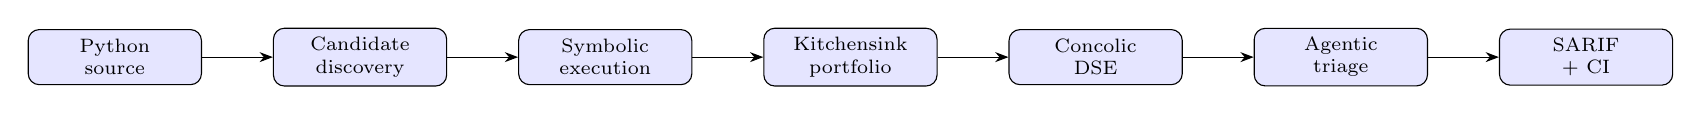
\begin{tikzpicture}[node distance=0.9cm,
  box/.style={draw, rounded corners, fill=blue!10, font=\scriptsize, align=center, minimum width=2.2cm,minimum height=0.7cm}]
  \node[box] (src) {Python\\source};
  \node[box, right=of src] (disc) {Candidate\\discovery};
  \node[box, right=of disc] (sym) {Symbolic\\execution};
  \node[box, right=of sym] (kit) {Kitchensink\\portfolio};
  \node[box, right=of kit] (dse) {Concolic\\DSE};
  \node[box, right=of dse] (tri) {Agentic\\triage};
  \node[box, right=of tri] (sarif) {SARIF\\+ CI};
  \foreach \a/\b in {src/disc, disc/sym, sym/kit, kit/dse, dse/tri, tri/sarif} {\draw[-{Stealth}] (\a) -- (\b);}
\end{tikzpicture}}%
\end{center}
\begin{itemize}
  \item \textbf{Discovery}: 67+ bug type checkers flag candidates
  \item \textbf{Symbolic execution}: build \(\sigma = (\text{pc}, \rho, h, \tau, \kappa, e, \Phi)\) and Z3 queries
  \item \textbf{Kitchensink}: guard check $\to$ AI $\to$ barrier $\to$ IC3 $\to$ CEGAR
  \item \textbf{DSE}: confirm TPs concretely
  \item \textbf{Triage}: LLM assigns severity with grounded reasoning
  \item \textbf{CI}: ratchet policy enforces monotonic improvement
\end{itemize}
\end{frame}

\begin{frame}{168. Slide 1: deliverable framing --- what to say}
\begin{itemize}
  \item The talk opens with the \textbf{deliverable}: a working system that finds real security and reliability bugs with formal elimination of false positives
  \item What to emphasise:
    \begin{itemize}
      \item Not a prototype, not a paper claim --- a system that produced SARIF records for real code
      \item The key differentiator: evidence-backed results (proofs or witnesses), not just heuristic suspicion
    \end{itemize}
  \item Avoid: ``we formulate the problem as\ldots'' --- that is the wrong register for RISE; lead with what ships
  \item Vocabulary you now know: SARIF, TP/FP, barrier certificate, SMT proof
\end{itemize}
\end{frame}

\begin{frame}{169. Slide 11: state tuple --- what to say}
\begin{itemize}
  \item When presenting \(\sigma = (\text{pc}, \rho, h, \tau, \kappa, e, \Phi)\):
    \begin{itemize}
      \item \textit{pc}: ``which line of bytecode is next''
      \item \textit{$\rho$}: ``what each variable symbolically equals''
      \item \textit{h}: ``the heap --- objects and their fields''
      \item \textit{$\tau$}: ``what type each object actually is''
      \item \textit{$\kappa$}: ``taint level --- did this value come from a user?''
      \item \textit{e}: ``any pending exception currently propagating''
      \item \textit{$\Phi$}: ``the accumulated constraints that got us here''
    \end{itemize}
  \item Say: ``this 7-tuple is the full world-state from which the verifier reasons''
\end{itemize}
\end{frame}

\begin{frame}{170. Slide 13b: barrier obligations --- what to say}
\begin{itemize}
  \item When you show the three obligations:
    \begin{enumerate}
      \item ``Initiation: when the function starts, we're already inside the safe zone''
      \item ``Consecution: every step of the program keeps us inside the safe zone'' --- stress: this is what we check for every loop iteration
      \item ``Separation: the safe zone never overlaps the bug condition''
    \end{enumerate}
  \item The ``fence'' metaphor works well for RISE: ``we build a mathematical fence around safe states; no execution can jump over it''
  \item If someone asks ``what if the fence can't be built?'': say ``we escalate to IC3/PDR which builds a clause-based version''
\end{itemize}
\end{frame}

\begin{frame}{171. Slides 13c--13g: the 20-paper map --- what to say}
\begin{itemize}
  \item These slides show how A3 connects to 20 foundational papers across 5 groups
  \item You don't need to explain every paper --- pick 1--2 per group and explain the connection
  \item Group by narrative:
    \begin{itemize}
      \item ``Stengle and Parrilo give us the math'' (SOS, Positivstellensatz)
      \item ``IC3/Bradley and SeaHorn give us the algorithm'' (clause-based, CHC)
      \item ``SLAM and BLAST give us the engineering'' (industrial-scale CEGAR)
      \item ``Houdini and ICE give us the synthesis'' (learning invariants)
      \item ``DART/KLEE give us the witnesses'' (concolic confirmation)
    \end{itemize}
\end{itemize}
\end{frame}

\begin{frame}{172. Handling expert questions: 5 common questions at RISE}
\begin{enumerate}
  \item \textbf{``Why polynomial certificates and not just abstract interpretation?''}\\
    --- AI widening is imprecise; barriers give exact proofs with checker certificates
  \item \textbf{``How do you handle unknown Python library calls?''}\\
    --- Conservative abstraction: treat return as unconstrained symbolic value; UNKNOWN routing
  \item \textbf{``What is your FP rate on open-source projects?''}\\
    --- Reference the evaluation section; quote the observed FP reduction percentage
  \item \textbf{``How does your SOS approach handle integers (discrete)?''}\\
    --- Integer intervals embedded in reals; integer assertions discharged by linear arithmetic first
  \item \textbf{``Does this scale to 100k LOC?''}\\
    --- Modular: analyse per-function; interprocedural via summaries; CI run on incremental changes
\end{enumerate}
\end{frame}

\begin{frame}{173. Terminology cheat sheet: what each term means in a sentence}
\begin{itemize}
  \item \textbf{Barrier certificate}: ``a polynomial function that acts as a mathematical fence,
    proved to exclude the unsafe states from the reachable set''
  \item \textbf{Consecution}: ``the mathematical condition ensuring the program cannot escape the safe zone in one step''
  \item \textbf{Concolic execution}: ``running the program with concrete inputs while simultaneously tracking symbolic expressions, to confirm bugs without path explosion''
  \item \textbf{SOS}: ``a way of proving a polynomial is always non-negative by expressing it as a sum of squares---the computationally tractable certificate form''
  \item \textbf{CHC}: ``Horn clauses encoding program transitions---the language in which we ask Z3 to find a loop invariant''
\end{itemize}
\end{frame}

\begin{frame}{174. Terminology cheat sheet (continued)}
\begin{itemize}
  \item \textbf{CEGAR}: ``iteratively refine an abstract program model using the counterexamples that expose its imprecision''
  \item \textbf{IC3/PDR}: ``incrementally build a sequence of tightening invariant frames until two frames are identical---that's your inductive proof''
  \item \textbf{Interpolant}: ``the minimal shared reason why two parts of a program formula are contradictory---used to extract new predicates for CEGAR refinement''
  \item \textbf{CI ratchet}: ``a policy that allows the security posture to only improve: once a bug is fixed, it can never reappear without breaking the build''
  \item \textbf{Kitchensink}: ``the ordered portfolio of verification methods tried for each candidate---cheapest first, escalating until a decision is reached''
\end{itemize}
\end{frame}

\begin{frame}{175. Pre-talk confidence: the two-sentence summary of each method}
\begin{itemize}
  \item \textbf{Path condition check}: find the constraints the program must satisfy to reach the bug; if they are contradictory (UNSAT), the bug is impossible.
  \item \textbf{Barrier certificate}: find a polynomial that stays positive in safe states and negative in unsafe ones; prove that program transitions can never push it from positive to negative (consecution).
  \item \textbf{CEGAR}: abstract the program coarsely; if the abstract model shows a bug, check if it is real; if not, learn why and tighten the abstraction.
  \item \textbf{IC3/PDR}: block bad states one by one, propagating blocking clauses backward through frames until the frames stabilise into a full invariant.
  \item \textbf{Concolic}: start with a concrete input from the solver; run the program while tracking symbolic constraints; confirm the bug is hit, or detect that the path diverges.
\end{itemize}
\end{frame}

%% ============================================================
%%  CHAPTER 12 — Reference Glossary
%% ============================================================

\begin{frame}{Chapter 12: Comprehensive Glossary}
\begin{block}{How to use this chapter}
These final slides define every term that appears in the A3 walkthrough.
Use them for quick reference before or during the talk.
\end{block}
\end{frame}

\begin{frame}{176. Glossary: A}
\begin{description}[Abstract interpretation]
  \item[Abstract interpretation] Analysis technique that approximates program semantics over an abstract domain (intervals, polyhedra, etc.) rather than concrete values.
  \item[Abstraction] A simplified model of a program; over-approximate abstractions are sound.
  \item[Alert fatigue] Developer response of ignoring all alerts because too many are false positives.
  \item[Agentic triage] An LLM-agent layer that contextualises static analysis findings before reporting to developers.
\end{description}
\end{frame}

\begin{frame}[shrink=12]{177. Glossary: B--C}
\begin{description}[Barrier certificate]
  \item[Barrier certificate] A function $B$ satisfying init, consecution, and separation obligations, certifying program safety.
  \item[Basic block] Maximal straight-line code sequence with single entry and exit.
  \item[CEGAR] Counterexample-guided abstraction refinement: iterative abstraction tightening.
  \item[CFG] Control flow graph --- nodes are basic blocks, edges are possible control transfers.
  \item[CHC] Constrained Horn Clauses --- logical encoding of program transitions used in CHC solvers.
  \item[CI ratchet] Continuous-integration policy allowing only security improvement, never regression.
  \item[Clause] A disjunction of literals; the atomic unit of SAT/IC3 invariant construction.
  \item[Concolic] Concrete + symbolic execution running simultaneously; DART/KLEE style.
  \item[Consecution] The inductive step of a safety proof: the safe zone is closed under transitions.
  \item[Craig interpolant] A formula derived from an UNSAT proof, used to extract new predicates.
\end{description}
\end{frame}

\begin{frame}{178. Glossary: D--I}
\begin{description}[DSOS]
  \item[DSOS] Diagonally dominant SOS: a linear-programming relaxation of SOS certificates.
  \item[DSE] Dynamic symbolic execution; a.k.a. concolic testing.
  \item[False negative (FN)] A real bug that was missed by the analyser.
  \item[False positive (FP)] A flagged candidate that is not a real bug; eliminated by proof.
  \item[Houdini] Algorithm that finds the maximal inductive conjunction of given candidate predicates.
  \item[ICE learning] Invariant learning via implication counterexamples; combines examples and SMT.
  \item[IC3/PDR] Frame-based invariant builder; property directed reachability.
  \item[Inductive invariant] A set $I$ satisfying initiation, consecution, and separation.
  \item[Interpolant] See \textit{Craig interpolant}.
\end{description}
\end{frame}

\begin{frame}{179. Glossary: K--P}
\begin{description}[k-induction]
  \item[k-induction] Inductive proof using the last $k$ states as the hypothesis.
  \item[Kitchensink] A3's ordered portfolio of verification methods tried for each candidate.
  \item[Liveness property] A property asserting something good eventually happens (not targeted by A3).
  \item[Path condition $\Phi$] Conjunction of branch constraints accumulated during symbolic execution.
  \item[PDR] Property directed reachability; same algorithm as IC3.
  \item[Positivstellensatz] Algebraic certificate theorem connecting polynomial positivity to SOS decompositions over semialgebraic sets.
  \item[Predicate abstraction] Abstract state represented as a boolean vector of predicate truth values.
\end{description}
\end{frame}

\begin{frame}{180. Glossary: R--Z}
\begin{description}[Reachability]
  \item[Reachability] The question: ``can the program reach a bad state?''
  \item[Safety property] A property asserting nothing bad ever happens; modelled as unsafe set $U$.
  \item[SARIF] Static Analysis Results Interchange Format; structured JSON for analysis findings.
  \item[SAT] Satisfiable: a formula has at least one satisfying assignment.
  \item[SDP] Semidefinite program; the optimisation problem arising from SOS certificate synthesis.
  \item[SMT] Satisfiability modulo theories; SAT extended with arithmetic, arrays, etc.
  \item[Soundness] If the analyser says safe, it is safe (no false negatives).
  \item[SOS] Sum of squares; certificate of polynomial non-negativity enabling SDP synthesis.
  \item[State tuple $\sigma$] A3's 7-tuple $(\text{pc}, \rho, h, \tau, \kappa, e, \Phi)$ characterising all analysis state.
  \item[Taint analysis] Tracking whether data flows from untrusted sources to dangerous sinks.
  \item[UNSAT] Unsatisfiable: no assignment makes the formula true; used as FP-elimination proof.
  \item[Z3] Microsoft's open-source SMT solver; primary decision procedure in A3.
\end{description}
\end{frame}

\begin{frame}[shrink=8]{181. Key equations at a glance}
\begin{align*}
&\textbf{Safety goal:} && R \cap U = \varnothing \\
&\textbf{Inductive invariant:} && S_0 \subseteq I,\; I \text{ closed under }T,\; I \cap U = \varnothing \\
&\textbf{Barrier obligations:} && \forall s\!\in\!S_0: B(s)\!\ge\!\epsilon,\;\forall (s,s')\!\in\!T: B(s)\!\ge\!0\!\Rightarrow\!B(s')\!\ge\!0,\;\forall s\!\in\!U: B(s)\!\le\!-\epsilon \\
&\textbf{Consecution check:} && I(s) \wedge T(s,s') \wedge \neg I(s') \text{ is UNSAT} \\
&\textbf{FP elimination:} && \Phi(\sigma) \wedge U_t(\sigma) \text{ is UNSAT} \\
&\textbf{TP witness:} && \Phi(\sigma) \wedge U_t(\sigma) \text{ is SAT, model confirmed by concolic}
\end{align*}
\end{frame}

\begin{frame}{182. Dependency map: which ideas build on which}
\begin{center}
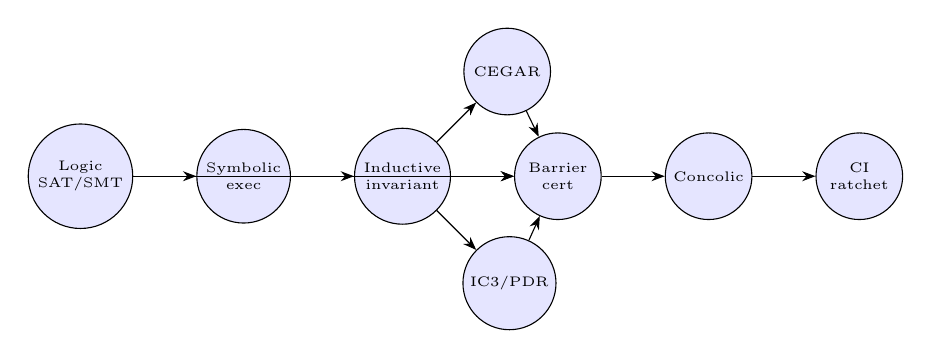
\begin{tikzpicture}[node distance=0.8cm,
  c/.style={draw,circle,fill=blue!10,font=\tiny,inner sep=2pt,minimum size=1.1cm,align=center}]
  \node[c] (logic) {Logic\\SAT/SMT};
  \node[c, right=of logic] (symex) {Symbolic\\exec};
  \node[c, right=of symex] (inv) {Inductive\\invariant};
  \node[c, right=of inv] (barrier) {Barrier\\cert};
  \node[c, above right=0.5cm and 0.5cm of inv] (cegar) {CEGAR};
  \node[c, below right=0.5cm and 0.5cm of inv] (ic3) {IC3/PDR};
  \node[c, right=of barrier] (conc) {Concolic};
  \node[c, right=of conc] (ci) {CI\\ratchet};
  \foreach \a/\b in {logic/symex, logic/inv, symex/barrier, inv/barrier, inv/cegar, inv/ic3, barrier/conc, cegar/barrier, ic3/barrier, conc/ci} {\draw[-{Stealth},thin] (\a) -- (\b);}
\end{tikzpicture}
\end{center}
\begin{itemize}
  \item Logic and symbolic execution are prerequisites for everything
  \item Inductive invariants are the central concept; barrier, CEGAR, and IC3 are all implementations
\end{itemize}
\end{frame}

\begin{frame}{183. The 10 questions to ask yourself before the talk}
\begin{enumerate}
  \item Can I explain consecution in one sentence without notes?
  \item Can I say why UNSAT eliminates a false positive?
  \item Can I describe barrier certificates as a ``level-set fence''?
  \item Can I explain what SAT + concolic confirmation means?
  \item Can I sketch the kitchensink portfolio order?
  \item Can I say what the CI ratchet policy does?
  \item Can I handle the question ``why not just test more?''?
  \item Can I explain why UNKNOWN is handled conservatively?
  \item Can I connect IC3/PDR to the frame-based invariant idea?
  \item Can I say what Z3 returns and what each result means?
\end{enumerate}
\end{frame}

\begin{frame}{184. What you \textit{don't} need to memorise}
\begin{itemize}
  \item The exact paper proofs of Positivstellensatz or Stengle's theorem
  \item The internal algorithm of Z3's Spacer CHC solver
  \item The precise SDP formulation for degree-4 barrier certificates
  \item The Hoare logic inference rules for compound statements
  \item The precise definition of the Galois connection in abstract interpretation
\end{itemize}
\begin{block}{Rule of thumb}
For every concept: know the \textbf{one-sentence intuition} and the \textbf{consequence for A3}.
You do not need to be able to implement it from scratch.
\end{block}
\end{frame}

\begin{frame}{185. The ``so what'' for each method}
\begin{itemize}
  \item \textbf{SMT/Z3 UNSAT}: ``so what'' --- false positives are eliminated with a mathematical proof
  \item \textbf{Barrier certificates}: ``so what'' --- loops are handled rigorously; not just unrolled
  \item \textbf{CEGAR}: ``so what'' --- when simple proofs fail, we iteratively improve the model until one succeeds or a real bug is confirmed
  \item \textbf{IC3/PDR}: ``so what'' --- an alternative invariant search that works even when polynomial templates fail
  \item \textbf{Concolic}: ``so what'' --- surviving candidates that look like real bugs are confirmed with a concrete input you can hand to a developer
  \item \textbf{CI ratchet}: ``so what'' --- this is not a one-time audit; it's a continuously enforced safety monotonicity property
\end{itemize}
\end{frame}

\begin{frame}{186. Practice: describe the pipeline to a non-expert}
\begin{block}{Your elevator pitch}
``We run Python code through a tool that symbolically explores all possible inputs simultaneously.
When it finds a potential crash or security hole, it either mathematically proves the problem can't
actually happen (in which case we discard it), or it finds the exact input that triggers it (in which
case we report it with a reproducible test case). The whole thing runs in CI so the codebase can
only get safer with each commit.''
\end{block}
\begin{itemize}
  \item This covers: symbolic execution, barrier elimination, concolic confirmation, CI ratchet
  \item No technical jargon needed for this version
  \item For RISE: expand each phrase with the technical detail from this primer
\end{itemize}
\end{frame}

\begin{frame}{187. Practice: describe the pipeline to a verification expert}
\begin{block}{Expert pitch}
``We encode Python semantics as a symbolic transition system over a 7-tuple state.
Candidates are discharged by SMT UNSAT (path-level) or inductive barrier certificates (loop-level)
synthesised via SOS/SDP. Residual unknowns go through an IC3-style clause learner and CEGAR predicate
refinement. TP survivors are confirmed concolicly via negation of SAT model constraints. Findings
are reported as SARIF with attached Positivstellensatz certificates or concolic traces; the CI
ratchet enforces monotonic security improvement.''
\end{block}
\end{frame}

\begin{frame}{188. Common misconceptions to correct}
\begin{itemize}
  \item ``\textbf{Symbolic execution always causes path explosion}'' --- No: A3 manages this with loop invariants and bounded unrolling; concolic avoids it by following one path
  \item ``\textbf{SMT can always give a definitive answer}'' --- No: UNKNOWN is a valid output; undecidable fragments exist
  \item ``\textbf{Formal verification means no false positives and no false negatives}'' --- No: A3 is sound-ish (aims for low FN) but not perfect; explicit UNKNOWN handling
  \item ``\textbf{Barrier certificates require the program to have polynomial data flow}'' --- Partially true: nonlinear programs need higher-degree templates; complex heap uses conservative abstractions
\end{itemize}
\end{frame}

\begin{frame}{189. The connection to control theory (for control engineers in RISE)}
\begin{itemize}
  \item Barrier certificates were invented in control theory (Prajna \& Jadbabaie, 2004) for continuous dynamical systems
  \item The discrete program version mirrors the continuous version: replace \(\dot{B}(x) \ge 0\) with \(B(x_{k+1}) \ge 0 \text{ if } B(x_k) \ge 0\)
  \item A RISE audience may include control engineers who know Lyapunov functions --- barrier certs are their safety analog
  \item Lyapunov functions prove \textbf{stability} (convergence to set); barrier certificates prove \textbf{safety} (avoidance of bad set)
  \item Key distinction: Lyapunov decreases globally; barrier only needs to stay non-negative, not decrease
\end{itemize}
\end{frame}

\begin{frame}{190. The connection to formal methods (for FM researchers in RISE)}
\begin{itemize}
  \item RISE may include formal methods researchers who know model checking, Alloy, TLA+
  \item A3 is an \textbf{automated program verifier} (like SLAM, CBMC, CPAchecker) for Python
  \item Key distinctions from classical model checking:
    \begin{itemize}
      \item Works on real source code, not specifications
      \item Uses polynomial certificates (not just SAT-based BDD model checking)
      \item Targets bug \emph{categories} (67+ types) rather than one property at a time
      \item Pairs proofs with concolic witnesses for actionability
    \end{itemize}
  \item If asked about completeness: A3 is not complete (UNKNOWN outcomes exist); the goal is high-confidence coverage, not exhaustive proof
\end{itemize}
\end{frame}

\begin{frame}{191. The confidence interval question}
\begin{itemize}
  \item RISE: ``What does a confidence interval of [0.7, 0.9] mean operationally?''
  \item It means: the Bayesian posterior weight on ``this is an exploitable bug in production'' is between 0.7 and 0.9
  \item The width of the interval reflects uncertainty about the model (how well our symbolic semantics mirrors the runtime)
  \item A narrow interval [0.85, 0.90] = highly calibrated estimate; a wide one [0.2, 0.8] = high uncertainty, needs more investigation
  \item The CI ratchet threshold is configurable: by default, block on confidence > 0.75; surface for review on confidence > 0.5
\end{itemize}
\end{frame}

\begin{frame}{192. Things the talk does NOT need to cover}
\begin{itemize}
  \item Full proof of soundness of the symbolic semantics (too long; refer to technical report)
  \item Every SDP solver parameter and tuning option (irrelevant to RISE audience)
  \item The implementation language and testing framework for A3 itself (Python + pytest)
  \item Precise performance benchmarks on every BugsInPy project (have the numbers ready but don't recite them)
  \item Comparison to every commercial SAST tool (stick to scientific comparators: Infer, CBMC, CPAchecker)
\end{itemize}
\end{frame}

\begin{frame}{193. Last-minute memory devices}
\begin{itemize}
  \item \textbf{Barrier = fence}: three nails --- Init (post in ground), Consec (fence is solid), Sep (fence excludes danger zone)
  \item \textbf{CEGAR = ABCs}: Abstract, Bug check, refine if Counterexample is Spurious
  \item \textbf{IC3 = tightening rings}: each frame is a tighter ring around the reachable states; when two rings coincide, you have the invariant
  \item \textbf{Concolic = GPS}: start from solver directions, drive concretely, check if you arrive at the bug
  \item \textbf{UNSAT = alibi}: the formula has no witness to the crime --- the bug is provably impossible
\end{itemize}
\end{frame}

\begin{frame}{194. Quick quiz: test yourself}
\begin{enumerate}
  \item What are the three barrier certificate obligations? \textit{(Init, Consecution, Separation)}
  \item What does Z3 return when a bug is provably unreachable? \textit{(UNSAT)}
  \item What is a spurious counterexample? \textit{(A CE in the abstract model with no real execution trace)}
  \item What does ``concolic'' stand for? \textit{(concrete + symbolic)}
  \item What does the CI ratchet prevent? \textit{(Security regression: only improvement allowed)}
  \item What is consecution? \textit{(The inductive step: safe zone closed under transitions)}
  \item What is SOS used for in A3? \textit{(Certifying barrier certificate non-negativity via SDP)}
  \item What does UNKNOWN mean as a solver result? \textit{(Undecided; handled conservatively by retaining candidate)}
\end{enumerate}
\end{frame}

\begin{frame}{195. The three sentences that tie the whole talk together}
\begin{block}{Opening hook}
``Every Python project ships with invisible bugs. We built a system that can prove they don't exist
--- or prove they do, with a reproducible trace.''
\end{block}
\begin{block}{Middle bridge (after Episode II)}
``What unifies all the methods is one idea: find a mathematical fence around the safe states and prove that
no execution can cross it. Barrier certificates are one way to build that fence; IC3/PDR and CEGAR are others.''
\end{block}
\begin{block}{Closing claim}
``The CI ratchet turns this from a one-time scan into a monotonicity property: every commit either
maintains or improves the security posture, backed by formal evidence.''
\end{block}
\end{frame}

\begin{frame}{196. The most important slide in the deck (13b)}
\begin{itemize}
  \item Slide 13b shows the three barrier obligations as the unifying interface
  \item \textbf{This is the intellectual core of the talk}: every method in the kitchensink is trying to satisfy these three conditions
  \item Practise explaining this slide until it feels natural:
    \begin{enumerate}
      \item Point at ``Init'' --- say: ``initial states are inside the fence''
      \item Point at ``Consec'' --- say: ``every step keeps us inside the fence''  
      \item Point at ``Sep'' --- say: ``the fence never overlaps the unsafe zone''
      \item Pause, then say: ``if we can find a certificate \(B\) satisfying all three, the bug is provably impossible''
    \end{enumerate}
  \item If you nail slide 13b, the rest of the talk follows naturally
\end{itemize}
\end{frame}

\begin{frame}{197. Appendix: key papers by theme}
\begin{description}[Control-theory origin]
  \item[Control-theory origin] Prajna \& Jadbabaie 2004 (HSCC), Prajna 2007 (TAC)
  \item[SOS foundations] Shor 1987, Parrilo 2000 (thesis), Lasserre 2001, Stengle 1974
  \item[Tractable relaxations] Ahmadi/DSOS 2019, Waki sparsity, Ames/CBF
  \item[Clause-based invariants] Bradley IC3 2011, Een/PDR 2011, SeaHorn/Gurfinkel 2015
  \item[Predicate abstraction] Ball/SLAM 2002, Henzinger/BLAST 2002, McMillan interpolants 2003
  \item[Invariant synthesis] Flanagan/Houdini 2001, Garg/ICE 2014, Alur/SyGuS 2013
  \item[Concolic testing] Godefroid/DART 2005, Cadar/KLEE 2008, Godefroid/SAGE 2012
\end{description}
\end{frame}

\begin{frame}{198. Appendix: A3 modules and their techniques}
\begin{center}
\begin{tabular}{lll}
\textbf{Module} & \textbf{Technique} & \textbf{Chapter} \\ \hline
\texttt{SymbolicExecutor} & Symbolic execution + Z3 & Ch 3, 4 \\
\texttt{BarrierSolver} & SOS/SDP barrier synthesis & Ch 6 \\
\texttt{IC3Solver} & IC3/PDR clause learning & Ch 7 \\
\texttt{CEGARLoop} & Predicate abstraction + interpolants & Ch 7 \\
\texttt{DSEEngine} & Concolic DSE confirmation & Ch 8 \\
\texttt{HoudiniSolver} & Houdini max-inductive conjunct & Ch 9 \\
\texttt{ConfidenceModel} & Bayesian evidence combination & Ch 10 \\
\texttt{TriageAgent} & LLM-based contextual triage & Ch 10 \\
\texttt{CIRatchet} & SARIF diff + CI enforcement & Ch 10 \\
\end{tabular}
\end{center}
\end{frame}

\begin{frame}{199. Final checklist before the talk}
\begin{itemize}
  \item[$\square$] I can say ``consecution'' confidently and explain it in one sentence
  \item[$\square$] I can explain why UNSAT = false positive elimination
  \item[$\square$] I can describe barrier certificates as a ``mathematical fence''
  \item[$\square$] I can sketch the kitchensink portfolio order (5 methods)
  \item[$\square$] I can explain the CI ratchet in one sentence
  \item[$\square$] I know what SARIF is and why it matters
  \item[$\square$] I have answers ready for the 5 common RISE questions (slide 172)
  \item[$\square$] I have practised slides 13b (barrier obligations) and 167 (full pipeline)
  \item[$\square$] I can connect to control theory if a controls person asks
  \item[$\square$] I have the opening hook memorised (slide 195)
\end{itemize}
\end{frame}

\begin{frame}{200. You are ready}
\begin{block}{What you now know}
\begin{itemize}
  \item Ch 1--2: Verification, safety, reachability, logic, SMT/Z3
  \item Ch 3--4: Symbolic execution, CFGs, state tuple, transition systems
  \item Ch 5: Inductive invariants, consecution, k-induction
  \item Ch 6: Barrier certificates, SOS, SDP, DSOS
  \item Ch 7: CEGAR, IC3/PDR, interpolants, abstract interpretation
  \item Ch 8: Concolic execution, DSE, witness confirmation
  \item Ch 9: Invariant synthesis --- Houdini, ICE, SyGuS
  \item Ch 10--11: Confidence scoring, triage, CI ratchet, full pipeline
  \item Ch 12: Glossary and quick reference
\end{itemize}
\end{block}
\begin{center}
\textbf{Good luck with the presentation.}
\end{center}
\end{frame}

%% ---- END OF CHUNK 4 (slides 141-200) ----

\end{document}
